% Template for a Computer Science Tripos Part II project dissertation
\documentclass[12pt,a4paper,twoside,openany]{report}
\usepackage[pdfborder={0 0 0}]{hyperref}    % turns references into hyperlinks
\usepackage[margin=25mm]{geometry}  % adjusts page layout
\usepackage[dvipsnames]{xcolor}
\usepackage{graphicx}  % allows inclusion of PDF, PNG and JPG images
\usepackage{verbatim}
\usepackage{pdfpages}
\usepackage{caption}
\usepackage{subcaption}
\usepackage{csvsimple}
\usepackage{longtable}
\usepackage{amssymb}
\usepackage{listings}
\usepackage{float}
\usepackage{forest}
\usepackage{hyperref}

% Code style
\definecolor{codegreen}{rgb}{0,0.6,0}
\definecolor{codegray}{rgb}{0.5,0.5,0.5}
\definecolor{codepurple}{rgb}{0.58,0,0.82}
\definecolor{backcolour}{rgb}{0.95,0.95,0.92}

\lstdefinestyle{mystyle}{
    backgroundcolor=\color{backcolour},   
    commentstyle=\color{codegreen},
    keywordstyle=\color{magenta},
    numberstyle=\tiny\color{codegray},
    stringstyle=\color{codepurple},
    basicstyle=\ttfamily\scriptsize,
    breakatwhitespace=false,         
    breaklines=true,                 
    captionpos=b,                    
    keepspaces=true,                 
    showspaces=false,                
    showstringspaces=false,
    showtabs=false,                  
    tabsize=2,
    xleftmargin=9pt,
    xrightmargin=9pt,
    frame=lines
}


\lstdefinelanguage{Kotlin}{
  comment=[l]{//},
  commentstyle={\color{gray}\ttfamily},
  emph={delegate, filter, first, firstOrNull, forEach, lazy, map, mapNotNull, println, return@},
  emphstyle={\color{OrangeRed}},
  identifierstyle=\color{black},
  keywords={abstract, actual, as, as?, break, by, class, companion, continue, data, do, dynamic, else, enum, expect, false, final, for, fun, get, if, import, in, interface, internal, is, null, object, override, package, private, public, return, set, super, suspend, this, throw, true, try, typealias, val, var, vararg, when, where, while},
  keywordstyle={\color{NavyBlue}\bfseries},
  morecomment=[s]{/*}{*/},
  morestring=[b]",
  morestring=[s]{"""*}{*"""},
  ndkeywords={@Deprecated, @JvmField, @JvmName, @JvmOverloads, @JvmStatic, @JvmSynthetic, Array, Byte, Double, Float, Int, Integer, Iterable, Long, Runnable, Short, String},
  ndkeywordstyle={\color{BurntOrange}\bfseries},
  sensitive=true,
  stringstyle={\color{ForestGreen}\ttfamily},
}

\lstset{style=mystyle}

\raggedbottom                           % try to avoid widows and orphans
\sloppy
\clubpenalty1000%
\widowpenalty1000%

\renewcommand{\baselinestretch}{1.1}    % adjust line spacing to make
                                        % more readable

\begin{document}

\bibliographystyle{plain}


%%%%%%%%%%%%%%%%%%%%%%%%%%%%%%%%%%%%%%%%%%%%%%%%%%%%%%%%%%%%%%%%%%%%%%%%
% Title


\pagestyle{empty}

\rightline{\LARGE \textbf{Charlie Maclean}}

\vspace*{60mm}
\begin{center}
\Huge
\textbf{Synthesis of Heart-Rate Detection Methods} \\[5mm]
Computer Science Tripos -- Part II \\[5mm]
King's College \\[5mm]
\today  % today's date
\end{center}

\newpage

\section*{Declaration}

I, Charlie Maclean of King's College, being a candidate for Part II of the 
Computer Science Tripos, hereby declare that this dissertation and the work 
described in it are my own work, unaided except as may be specified below, 
and that the dissertation does not contain material that has already been 
used to any substantial extent for a comparable purpose.

I am content for my dissertation to be made available to the students and staff
of the University. 

\bigskip
\leftline{Signed [signature]}

\medskip
\leftline{Date [date]}

%%%%%%%%%%%%%%%%%%%%%%%%%%%%%%%%%%%%%%%%%%%%%%%%%%%%%%%%%%%%%%%%%%%%%%%%%%%%%%
% Proforma, table of contents and list of figures

\pagestyle{plain}

\chapter*{Proforma}

{\large
\begin{tabular}{ll}
Candidate Number:               & \bf 2410C    	                   	\\
Project Title:      & \bf Synthesis of Heart-Rate Detection Methods	\\
Examination:        & \bf Computer Science Tripos -- Part II, July 2020 \\
Word Count:         & \bf 10,927					\\
Codebase Line Count:& \bf 4,119\footnotemark[1]				\\
Project Originator: & \bf Dr Robert Harle                   		\\
Supervisor:         & \bf Dr Robert Harle                   		\\ 
\end{tabular}
}
\footnotetext[1]{Own code, excluding blank lines.
}
\stepcounter{footnote}


\section*{Original Aims of the Project}

The sensors that detect heart-rate in smart-watches are unreliable,
particularly when running. This project aimed to design and implement methods
to calculate a more reliable heart-rate from the signals that are provided.

The project would include designing an application to run on the watch and
collect data, along with implementing a variety of filters to clean the
signal, and then creating methods to extract the heart-rate.

\section*{Work Completed}

The project fully met the proposal’s success criteria.

In the project, I designed an application to collect data; implemented and
tuned filters to remove noise; removed motion noise and detected heart-rate. I
then investigated using earbud sensors and how to merge signals from earbuds
and watches.

The end result is an algorithm to extract heart-rate from the watch and a
sensor-fusion algorithm which combines the best features of both the watch and
the earbuds, giving a heart-rate reading more accurate than either alone.

\section*{Special Difficulties}

None.
 

\tableofcontents

\listoffigures

\newpage
\section*{Acknowledgements}


%%%%%%%%%%%%%%%%%%%%%%%%%%%%%%%%%%%%%%%%%%%%%%%%%%%%%%%%%%%%%%%%%%%%%%%
% now for the chapters

\pagestyle{headings}

\chapter{Introduction}

Elite runners have historically used heart rate to provide an accurate 
measure of intensity, and allow them to train more effectively. 
Previously, Electrocardiography (ECG) chest straps have been 
used to measure heart rate, by detecting the electrical signals controlling 
the expansion and contraction of the heart. They are accurate devices however
often prohibitively expensive, and hence inaccessible to casual runners.

In recent years, a new technology has emerged - Photoplethysmogram (PPG) 
- light is directed at the skin, and blood volume changes caused by the
cardiac cycle are detected through the changes in the reflected light
intensity. PPG sensors are cheaper than ECG sensors, and hence are 
available in a variety of products, particularly smartwatches. Recently, some
wireless earbuds have been released containing PPG sensors as well. These 
innovations have bought a new wave of advanced training and monitoring into
the lives of many runners.

Switching from ECG to PPG is not without problems though - ECG sensors generally return a
clean signal, as opposed to PPG signals which are contaminated with
noise.

In particular when running, the motion can cause blood velocity to 
change, and the sensor can slip across the skin \cite{Wijshoff17}, 
\cite{Wood06}. These result in distortions to the PPG signal, known as a
motion artifacts (MAs). Fortunately, smartwatches contain other sensors, such
as accelerometers and gyroscopes which can assist in predicting the presence of 
MAs, and hence compensate for them.

My goal is to research and develop a heart rate detection algorithm
for smartwatches worn during running, and to demonstrate it is accurate.
Additionally, I would like to explore the use of earbuds with PPG sensors as
an alternative source of heart-rate. 



\chapter{Preparation}

This chapter details the steps I took to determine how to develop my
implementation. It first describes photoplethysmography, the method with which heart-beats are
detected on watches. Next,
I give an overview of some of the tools I may choose to use in my project:
filters and spectrums. Then, I take a look at some of the solutions to this
problem which have been proposed across a few papers. Finally I outline my
development methodology. 

\section{Photoplethysmography (PPG)}

To develop an algorithm to track heart-rate on wrist-watches it is first important to
understand how watches track heart activity. PPG is a technique where light is
used to detect the volume of blood in veins. In hospitals, this is used in
finger pulse oximeters (figure \ref{fig:fingerppg}) to record the heart-beat
of patients. These work by transmitting light on one side of the finger, and
then measuring how much light is received on the other side of the finger.
The amount of light which permeates through the finger is related to how much
blood is currently in the veins.


\begin{figure}[h!]
	\centerline{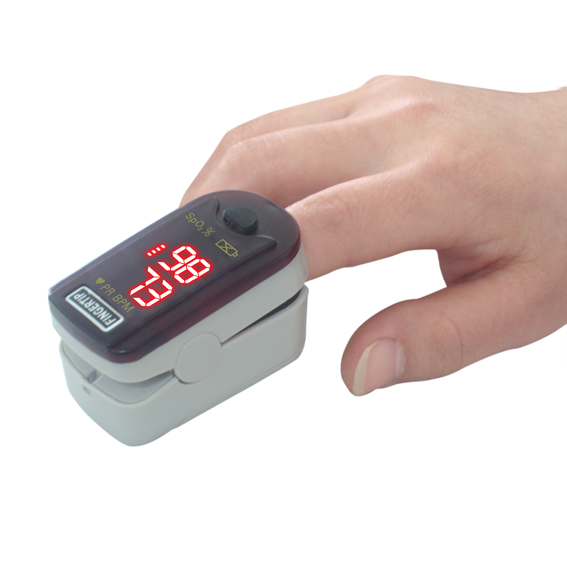
\includegraphics[width=0.3\textwidth]{figs/fingerppg.jpg}}
	\caption{Finger pulse oximeter. Image source \cite{wiki:fingerppg}.}
\label{fig:fingerppg}
\end{figure}

With watches, we cannot transmit light on one side, and
receive light on the other side, as the wrist is far too large. Hence, instead
of monitoring the absorption of light by the skin, we monitor the reflection
of light by the skin. A light is shone into the wrist, and sensors nearby
monitor how much is reflected back. When the wrist is full of blood, more
light is reflected back as blood scatters light.

We know now how the signals are recorded, but we have not yet explored the
signal that is actually received from this technique. In figure
\ref{fig:typicalppgsignal} we see a
clean PPG recording. There are two peaks in the data - a systolic peak and a
diastolic peak. The systolic peak represents the point at which the heart has
beat - and hence pushed blood through the body. The challenge is to find this
peak.

\begin{figure}[h!]
	\centerline{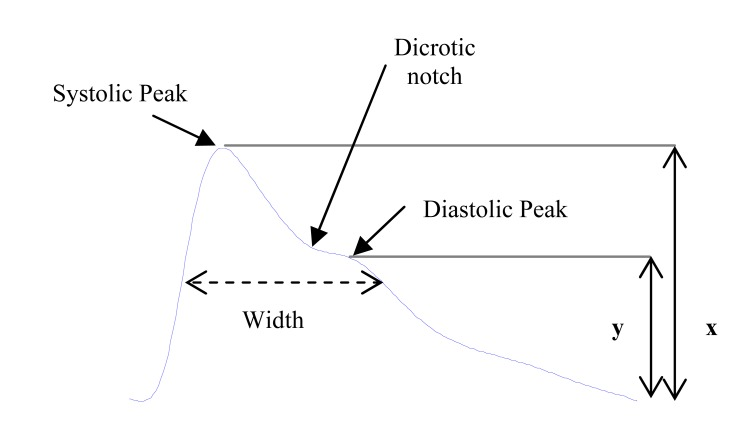
\includegraphics[width=0.7\textwidth]{figs/typicalppgsignal.jpeg}}
	\caption{Example PPG signal. Image and annotations from \cite{elgendi12}.}
\label{fig:typicalppgsignal}
\end{figure}

\section{Techniques}

In this section, I detail the techniques which I may find useful in my
implementation.

\subsection{Filtering} \label{sec:intro-filters}

PPGs produce a large amount of noise from various sources:
\begin{itemize}
	\item Light pollution. Both DC and AC lights in the environment can
		infiltrate the sensor, affecting the PPG signal \cite{kim15}.
	\item Temperature. As temperature increases, so does the volume of
		blood, which will be picked up by the PPG sensor 
		\cite{shin16}.
	\item Breathing. The change in pressure accosiated with respiration
		causes variations in the flow of blood, and hence can be seen
		by the PPG sensor \cite{allen02}.
\end{itemize}

In order to remove much of this noise, we can use filters to remove
frequencies we know are irrelevant. We know the heartbeat can vary from 
30 to 220 beats per minute, and hence we would like to disregard any
frequencies 
outside of this range. In this section, I will introduce the concept of 
filters.

\begin{figure}[h!]
	\centerline{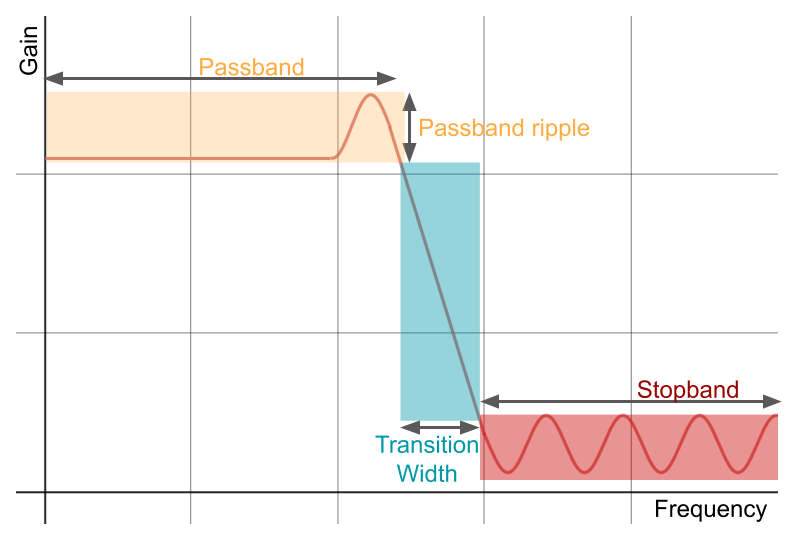
\includegraphics[width=0.8\textwidth]{figs/filter.png}}
\caption{Diagram showing filter characteristics}
\label{fig:filterdiag}
\end{figure}

Figure \ref{fig:filterdiag} displays an example filter magnitude response
diagram. This plots the amount of gain applied to each frequency. A gain of
zero means the signal is removed, a gain of one means the signal is unchanged.
The characteristics displayed are as follows.

The passband is the range of frequencies we would like to retain. In an ideal
filter, there is no loss within the passband.

Passband ripple describes the variation in amplitude \emph{within} the
passband. An ideal filter will have no passband filter, such that all
frequencies within the passband are permitted equally.

The transition width is the frequency range between the start and stop band.
Ideally, this is zero, such that frequencies outside of the passband are
instantly reduced.

The stopband is the range of frequencies we wish to remove. An ideal filter
completely removes all frequencies within the stopband.

There are four different filter types, which describe the frequencies we remove, as
follows:

\begin{itemize}
	\item Lowpass - allow frequencies below the critical frequency.

	\item Highpass - allow frequencies above the critical frequency.

	\item Bandpass - combination of lowpass and highpass - given two
		frequencies, we want the passband to be between those
		frequencies.

	\item Bandstop - given two frequencies, put the stopband between them,
		leaving the passband outside those frequencies.
\end{itemize}

\subsection{Spectrum}

A spectrum (or power spectrum) describes the power of each frequency present
within a signal.
This is a useful tool for analysing signals, giving us the ability to detect
where the frequency corresponding to heart-rate is, and additionally detect
what frequencies are noise in a signal.

To demonstrate a spectrum, I produced a signal of two sine waves, with
frequency 10 hz
and 30 hz, and some random noise. The spectrum this produced is shown in 
figure \ref{fig:example-spectrum}, it shows the presence of the two sine
waves, and the random noise is shown by the random baseline variation.

\begin{figure}[h]
	\centering
	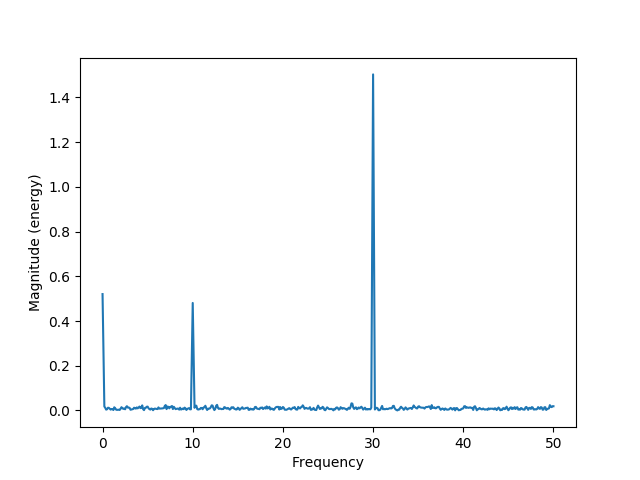
\includegraphics[width=0.5\textwidth]{figs/example-spectrum.png}
	\caption{An example spectrum.}
	\label{fig:example-spectrum}
\end{figure}



\section{Current Algorithms}

In this section, I look at the literature already produced on this topic,
discussing the algorithms which have been proposed in various papers.

\subsection{TROIKA}

TROIKA \cite{Zhang15} is a general framework for removing motion artifacts
from PPG signals taken when exercising. It consists of signal decomposiTion
, sparse signal RecOnstructIon and spectral peaK trAcking, each of which I will
explain here.

Signal decomposition is where a signal \(s\) is split into \(Q\) components
such that $s=\sum_1^Q s_i$. TROIKA recommends using singular spectrum analysis
(SSA) which decomposes the signal into oscillatory components and noise. It
determines what components are likely noise based on analysis of the frequency
spectrum of accelerometer data. The dominant frequencies in the accelerometer
signals are determined to be noise in the PPG signal.

Sparse signal reconstruction (SSR) is used to generate the frequency spectrum of the
now filtered PPG signal. As opposed to a periodogram, the spectrum from SSR
gives higher resolution frequency information, allowing more precise
identification of peaks.

Spectral peak tracking uses the current SSR spectrum, and the last known
heart-rate. In the paper, they use an 8 s window, with 2 s shifts, which means
the algorithm is run on one 8 s segment, before being shifted 2 s forwards then
run again.
The windows of the signal overlap by 6 s, meaning that the heart-rate
between two calculations will be very similar. Hence, TROIKA recommends
selecting a peak in a small range around the last known heart-rate.

\subsection{Finite State Machine}

The issue with the TROIKA framework is that it is prone to repeating errors
when they happen. For example, if the algorithm accidentally locks on to a frequency
related to motion it is very difficult to recover. A technique
suggested to avoid these errors makes use of finite state machines (FSM)
\cite{Chung19}.

This approach uses a FSM with four states as follows: 

\begin{itemize}
	\item Stable - the heart-rate estimate is likely to be very accurate.
	\item Recovery - the heart-rate estimate is somewhat accurate.
	\item Alert - the heart-rate estimate is possibly wrong.
	\item Uncertain - the heart-rate estimate is probably wrong.
\end{itemize}

To transition between states we need some sort of measure which tells us how
confident we are in the heart-rate estimation - in the FSM we use crest factor
(CF). The CF is the ratio of the peak value to the root-mean-squared value.
The lower the CF, the less likely the HR estimate is to be accurate. Hence,
when the CF value falls below some threshold, we go into a state with less
confidence in the heart-rate value. Additionally we are guided by heart-rate
change - if the heart-rate remains constant that is a sign we are locked on
the wrong signal.

Now, we have a FSM which will describe our confidence in a heart-rate
measurement - the question is how we use it. In the paper, an estimation is
only valid if it was taken in the
stable state. Hence, we sacrifice some of the data, but as a result we can be
much more confident in the results we do get.

\subsection{JOSS} \label{joss-intro}

JOSS \cite{Zhang15.2}, or JOint Sparse Spectrum reconstruction consists of two
stages, joint sparse spectrum reconstruction and spectral peak tracking. I
will explain these here.

Joint sparse spectrum reconstruction aims to produce a spectrum of the raw PPG
as though there were no MAs. It does this by simultaneously calculating the
power spectrums of the PPG signal and all the accelerometer channels. It then
subtracts the accelerometer channels spectrums from the PPG spectrum in such a
way that retains only the frequencies associated with heart-rate.

Spectral peak tracking is much the same as described in TROIKA, initially
finding the highest peak in the PPG spectrum. It then follows that peak using
the assumption that in two successive windows the heart-rate will be very
similar.

JOSS improves on TROIKA, providing a lower average absolute estimation error
and additionally works better when the PPG is sampled at a lower rate.


\subsection{PARHELIA}

PARHELIA \cite{Fujita18} is a PARticle filter-based algorithm for HEart rate
estimation using photopLethymographIc signAls. It consists of two stages:
spectral analysis, and then particle filtering, which I will delve into now.

The spectral analysis computes the spectrum of the PPG and each acceleration
signal, by running FFT on each. 

A particle filter can be used to represent uncertainty in a system, by having
multiple particles representing estimates of the current state. Each particle
is assigned a weight which represents our confidence in that particle being
correct. In PARHELIA, there are five steps, as follows:
\begin{enumerate}
	\item Initialisation - generate particles uniformly in the range 60
		bpm and 170 bpm.

	\item Prediction - every iteration, particles are moved randomly based on a normal
		distribution with standard deviation 6 bpm.

	\item Weight calculation - the weight of a particle is increased if
		its bpm is a peak in the PPG signal, and reduced if it's a
		peak in the accelerometer data.

	\item BPM Estimation - we estimate current BPM by looking at the
		weighted average of particles.

	\item Resampling - particles with the lowest weights are redistributed
		to more likely states.
\end{enumerate}

This approach improved on JOSS, claiming to provide 8.6\% better estimation
accuracy, and 20 times faster performance. However, it does require a higher
sampling rate than JOSS.



\section{Development Strategy}

I chose to implement the project in several stages:

\begin{enumerate}
	\item Develop the application to record and save PPG data taken while
		running, using Android Studio and Kotlin. I will then import the data
		into Python, which is widely used for data analysis as it's
		easy to produce terse code, and has several helpful
		libraries.

	\item Investigate the use of different filters to remove unwanted frequencies.

	\item Implement methods which will remove motion noise from the PPG
		signal. I may use the accelerometer, which provides a signal
		that is correlated to
		the motion noise.

	\item Develop algorithms which will calculate a heart-rate, given a
		PPG signal.

	\item Investigate joint sparse spectrum reconstruction as a heart-rate
		calculation technique (based on JOSS above).

	\item Research the use of earbuds as an alternative to wrist-based
		monitoring.

\end{enumerate}




\section{Starting Point}

The codebase is built from scratch, as per my proposal. The joint sparse
spectrum reconstruction method I implement is based on JOSS, as described in
my implementation (section \ref{sec:joss}).

\chapter{Implementation}

In this chapter, I describe the steps taken to create the system. I first
describe the implementation of a data gathering system, followed by details of
the algorithms I implement to calculate heart-rate from the data. At the end
I investigate a promising approach using sensor fusion with 
wrist-watches and earbuds.

\section{Gathering Data}

In this section I detail the process of developing an
application to record PPG data on a Wear OS watch. Wear OS is a version of
Android designed by Google for wearables. The development turned out to be more
complicated than I presumed due to interesting issues inherent with developing for a small
wearable with limited power.

\subsection{Wear OS Development}

\paragraph{Language Choices}

The watch application was developed using the official IDE for Android
development, Android Studio. I programmed in 
Kotlin, an open source language based on Java, which aims to
reduce boilerplate code, add null-safety, and remain interoperable with
Java. I had never used Kotlin before this, so first some time was spent
familiarising myself with the
language.

\paragraph{Structure}

The program was split into classes as described here:

\begin{itemize}
	\item \emph{MainActivity} - central class responsible for 
		recording and saving the data.

	\item \emph{SensorListener} - interface which overrides the Android
		\emph{SensorEventListener}. Contains methods which
		are called by the WearOS system whenever new sensor data comes
		in. Additionally has a method which saves the received data.
		We use one child for each sensor as each different sensor
		provides different data, and must be saved in a different
		format. So we have the following children:

	\begin{itemize}
		\item \emph{PpgListener}
		\item \emph{AccelerometerListener}
		\item \emph{RotationListener}
	\end{itemize}

\end{itemize}

When the user presses start recording, \emph{MainActivity} registers each
\emph{SensorListener} with the OS so they receive any sensor changes.
When the user presses stop recording, \emph{MainActivity} unregisters the
listeners and gets each one to save their recording.

\paragraph{Storing Recordings}

It was critical that I could easily import the recordings into any program, and
hence I chose to export the data into a CSV text file. I could have
alternatively used something with structure, such as JSON or XML, but the
data we are recording is very simple, containing identical records. CSV files
are widely supported, and can be easily imported into spreadsheet software
allowing me to quickly check that the program was working. Each \emph{Listener}
class uses a \emph{CSVWriter} object from library \emph{opencsv} to write to a
unique file for each sensor, within a directory chosen by \emph{MainActivity}.
For example, at the end of the recording in the directory
\emph{YYYY-MM-DD/HH.MM.SS/} we have files \emph{ppg.csv},
\emph{accelerometer.csv} and \emph{rotation.csv}.

\paragraph{Interface}

I chose a simple yet functional interface to allow the user to start and stop
a recording. The interface changes colour when recording, which makes it very
easy to verify the recording is in progress. See the interface in figure
\ref{fig:interface}.

\begin{figure}[tbh]
	\centerline{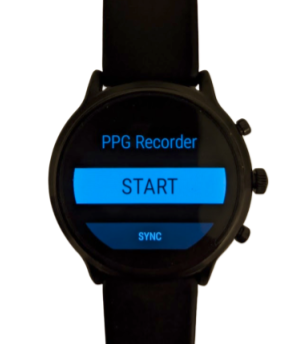
\includegraphics[width=0.2\textwidth]{figs/interface.png}}
	\caption{Watch Interface.}
	\label{fig:interface}
\end{figure}



\paragraph{Problems}

After I'd developed the application and was testing it out I found two key
issues which I will explain here.

\subparagraph{Power Saving}

Power is an enormous issue on wearable devices, as the form factor drastically
constrains the size of the battery. Hence developers have designed
Wear OS to limit power usage of any application as much as possible. 
As part of these optimisations Wear OS automatically suspends any application
it thinks is not being used. While this is useful for most users, my
application needs to run continuously without interruption.

Initially in testing there were long periods of time where no sensor values
were being recorded, due to the application being suspended.

To fix this issue, a wake lock was included. Once a wake lock is acquired, the
OS does not suspend the application. I added one which is acquired every time
a recording is started, and released when the recording ends. The following
code obtains the wake lock:

\begin{lstlisting}[language=Kotlin]
// Obtain a wakelock to ensure the listeners are active while updates are being provided
mWakeLock = (getSystemService(Context.POWER_SERVICE) as PowerManager).run {
	newWakeLock(PowerManager.PARTIAL_WAKE_LOCK, "ppgrecorder:ListenerLock").apply {
		acquire()
	}
}
\end{lstlisting}

\subparagraph{Sampling Rate}

When I subscribe to values from the PPG sensor and accelerometer sensors, the
API asks for a parameter - sampling period, which is the amount of delay we
want between sensor readings being delivered. In practice, Android only uses
this number as a hint - values may be provided at a higher or lower rate.

Additionally, Android does not expose the actual rate at which sensor values
are being provided to the OS. The sensors which are placed within devices
always have a constant sampling rate. Sensors write to a very short buffer,
which Android then reads from at a rate it decides. This means although we
have a reliable sensor, Android occasionally misses readings.

I record the data with a sampling period of 0 - which signifies that I want
updates as soon as they are available. However, Android is not guaranteed to
provide this. We need a constant sampling rate to work with in my programs, so I 
define sampling rate to be equal to the time difference
between the first and last sample, divided by the number of samples.

So, I have created an application which allows the user to record
accelerometer and PPG values at a constant sampling rate, then save them to
the watch.

\subsection{Uploading Recordings}

Now that data has been recorded, the values must be uploaded somewhere to enable
later analysis. I created a server which would run on a Raspberry Pi that the
watch could connect to over the local network. The files would be passed to
the server, and from there the files are uploaded to Google Drive where they
can be accessed anywhere. In this section I go over the details of this
implementation. See figure \ref{fig:upload} for the overall uploading process.

\begin{figure}[tbh]
	\centerline{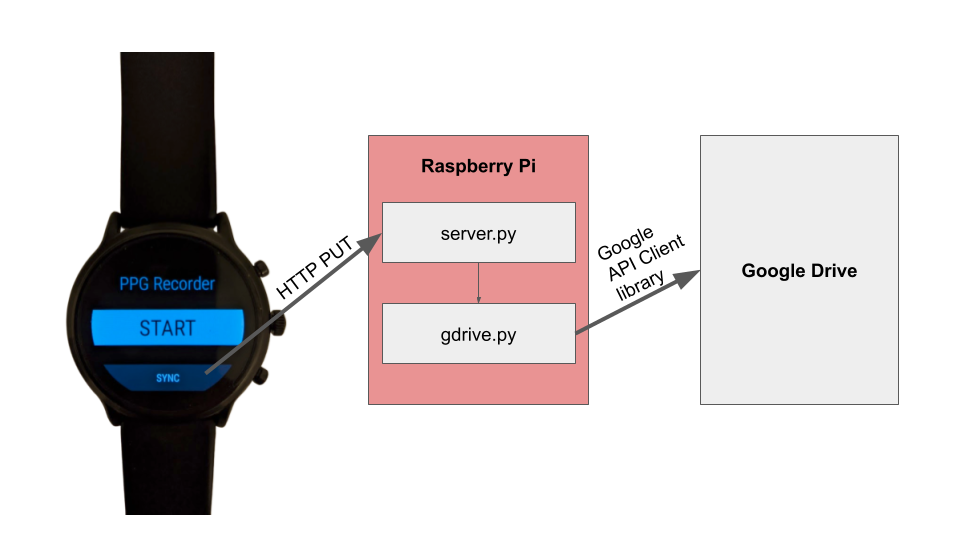
\includegraphics[width=0.7\textwidth]{figs/upload.png}}
	\caption{The overall process of uploading files.}
	\label{fig:upload}
\end{figure}

\subsubsection{Changes to Wear OS Application}

First a 'sync' button was included in the interface, which users can press to
trigger the sending of files to the server, as seen in figure
\ref{fig:interface}.

Then I added the logic to be triggered when the button is pressed. This logic
iterates through every file in the recordings directory and performs a HTTP
PUT request with them. I used the \emph{OkHttpClient} library in order to
send these requests.

\subsection{Raspberry Pi Access Point}

To connect the watch to the server I needed to create a local access point on the
Raspberry Pi. The
packages I used to do this were \emph{hostapd} and \emph{dnsmasq}. 

The package \emph{hostapd} is used to setup the access point, so I used it to
configure the
SSID and password it can be accessed on. 

The package \emph{dnsmasq} is used to setup the DHCP service, assigning IP
addresses to devices. I set it up to assign the range of adresses from 192.168.0.1 to
192.168.0.255 on the same interface as \emph{hostapd} is broadcasting over.

\subsubsection{Flask Web Application on Raspberry Pi}

Now, to setup the server I used Flask, a Python Web App framework. I chose
this over other frameworks like Django as it provides a flexible framework
which is easy to understand and deploy.

I created an application \emph{server.py} which
accepts PUT requests containing a file from URL \emph{/upload/path} where
\emph{path} is the location we want to place the file. Then, the server
makes the directories up to \emph{path} if they don't exist, placing the file
in this directory. 

Once the file has been saved, I upload the new file to google drive, by
calling \emph{gdrive.py}, which I detail below.

\subsubsection{Python Scripts to Upload to Google Drive}

To manage the process of uploading files to Google Drive, I created a new
application \emph{gdrive.py}. To upload to Google Drive using Python, I used
the library \emph{googleapiclient}, which was a surprisingly complicated API,
as I will explain here.

First, to connect to Google servers, the API must authenticate to ensure that
it has permission to access a user's Drive. The service requires a credential
token which expires periodically. Hence, I store the credentials in a binary
file using library \emph{pickle}, and when I need to access them, I 
refresh them if they have expired.

Then, I must actually upload a file. This process is complicated as Google
Drive does not use a path system to store files. Instead, it is a set of files
each with a unique IDs. A folder is simply a file with a \emph{folder} file
type, and a collection of files associated with it. Furthermore, as files are
not referenced by filename, it is possible to have multiple files in the same
folder with exactly the same filename.

The Google Drive API for Python only contains two methods which are useful for
my application:

\begin{itemize}
	\item \emph{list(parent)} which lists the files within folder
		\emph{parent}.

	\item \emph{create(file, metadata)} which creates a \emph{file} with
		\emph{metadata}. Note that as folders
		are just files, this is also how folders are created, by
		specifying the folder type in \emph{metadata}.
\end{itemize}

Using these methods, I define three methods within \emph{gdrive.py}, as follows:

\begin{itemize}
	\item \emph{createFolder(name, parent)} creates folder by creating a
		file with metadata specifying the type as a folder.

	\item \emph{getOrCreatePath(path)} is used to obtain a 'path' from Google
		Drive. It works by iterating through each level of the path,
		creating the necessary folders if they don't already exist,
		then entering them.

	\item \emph{uploadFile(filepath)} created the path up to the file
		given by filepath, and then upload the file to the folder.
\end{itemize}

Now, I have created a system which allows the user to upload recordings from
the watch to Google Drive via my server. And thus, I have completed the data
recording process. The data is recorded on the Wear OS app, and then with a
click transmitted to a Google Drive so it can be analysed.


\subsection{ECG}

In order to evaluate this project, I need to know my actual heart-rate. This
is done using a portable electrocardiogram (ECG) chest strap, the Bitium Faros
360. It sits on your chest, and records the voltage changes across the skin.
When your heart beats, the muscles within cause voltage spikes which are
picked up by the ECG. The device is setup with a configuration 
file, where I choose to enable
the accelerometer, and set the ECG to sample at a rate of 500 hz.

Once I have recorded something using the ECG 
each recording is saved as an EDF file, a format
designed for storing medical time series. I read the recordings into Python
by using the \emph{PyEDFlib} library.

To then calculate the heart-rate I use the Python library \emph{heartpy} which
has been developed to remove baseline variation and then calculate reliable
peak positions in the ECG signal.

\subsection{Synchronising Signals} \label{sec:sync}

Once I have collected the PPG signal from the watch, and have recorded the ECG
from the chest, I need a method to synchronise the signals, such that they
start at the same time and we can compare them accurately.

I set out to produce a solution with the following properties:
\begin{itemize}
	\item Able to synchronize signals with \(\pm0.3\)s accuracy. With a
		heartbeat of 200 bpm this represents being within a heartbeat.
		This is an acceptable level of delay, as heart rate is
		averaged over several beats anyway.

	\item Can synchronize signals given the two recordings are started
		within two minutes of each other. This constraint is helpful
		as it prevents wasted time searching through the signal.

	\item Does not use the clocks built into the device. We must assume
		the clock within the ECG is unreliable. Additionally, the two
		devices may be synchronized to different time, and hence could
		be out by any amount of time.
\end{itemize}

Given I know both devices have an accelerometer, I realised I could ask the
wearer to move in some motion which is picked up by both devices. Then, I
could compare the two accelerometer signals in order to discover the
movement. Then comparing the starting times of the two signals would enable
calculation of the time difference between them.

The type of motion I chose was important, as it had to be easy to explain to
the wearer, but also provide sufficient motion for it to be identifiable
against normal motion. I decided jumping was appropriate -
I would ask the wearer to hold the watch close to their chest and jump three
to five times.

The cross correlation of two signals \(f\) and \(g\) is a measure of
similarity as a function of the displacement between them. It is simple to
calculate, as a sum of the products between the samples of \(f\) and of \(g\)
displaced by \(n\).

To synchronise the accelerometer, I developed the following three step 
algorithm:
\begin{enumerate}
	\item Normalize signals, by moving to zero mean, 

	\item Crop PPG signals to two minutes, crop ECG signals to four
		minutes, compute cross correlation with \(f=\) PPG
		acceleration, \(g=\) ECG acceleration.

	\item Compute the other way - crop ECG to two minutes, PPG to four
		minutes, compute cross correlation with \(f=\) ECG
		acceleration, \(g=\) PPG acceleration. I compute both ways, to
		ensure that we can synchronise regardless of which device
		started recording first.

	\item Find the maximum cross correlation across each of the
		calculations.







\end{enumerate}

\subsection{Informed Synchronisation}

Running cross correlation on two signals is an effective way to compare their
similarity, however it is not efficient. Cross correlation has complexity
\(O(n^3)\). In this section I develop a new algorithm which uses knowledge of
the problem to speed up the cross correlation calculation.

By graphing the cross correlation of the acceleration signals, we can draw
some useful features that help us to work out a more optimal solution. See
figure \ref{fig:cross-correlation} for an example of absolute cross correlation plotted
between the two accelerometer signals over time. It is clear that there is one
peak which is above all the others, where the jumps line up perfectly.
However, in addition we can see that there is a significant rise in cross
correlation around the peak, where we are seeing peaks due to one or two of
the jumps aligning. This is useful as we do not need to scan at each
possible time difference, instead we can do an initial, lower resolution scan.
After this initial scan is done, we find the peak, and check each possible
time difference around the lower resolution peak to find the actual peak.

\begin{figure}[h!]
	\centerline{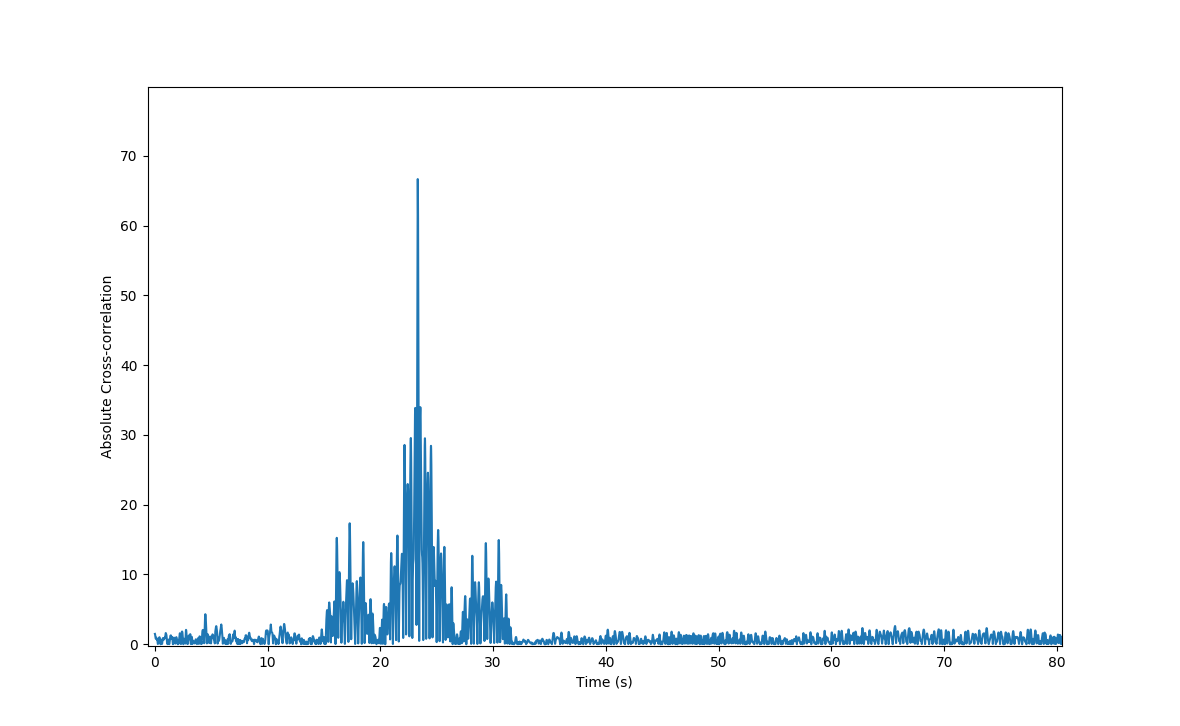
\includegraphics[width=0.8\textwidth]{figs/cross-correlation.png}}
	\caption{Absolute Cross Correlation over time. }
	\label{fig:cross-correlation}
\end{figure}

The algorithm I designed takes two parameters: step size (\emph{g}) and
correct range (\emph{r}). Step size is the number of samples we skip in the initial scan, so the
lower it is the more likely we are to find the peak but the longer the
algorithm takes. Correct range gives the range of the time period we want to
scan once we have found an initial peak, in order to find the actual peak. The
code is included here:
\begin{lstlisting}[language=Python]
def fast_correlate(f, g, freq, init_time_gap = 0.25, search_bound = 3):
    """
    Calculate cross correlation c of two numpy arrays, as defined by 
    c[k] = sum_n (f[n+k] * g[n]) using optimized method 
    which does an initial correlation at a lower resolution and then 
    hones in on the solution.

    Parameters
    ----------
    f, g : numpy arrays
    Input signals, resampled to ensure they're at the same frequency.

    freq : float
        The frequency of the signals.

    init_time_gap : float
        Interval at which to perform correlation initally in seconds. 

    search_bound : float
        Bound within which we search for the solution once we have made an initial pass.
        

    Returns
    -------
    k : int
        k is the time at which we think the signals are synced, given in terms of the number of samples through f we are.
        i.e. the value of k which maximizes c[k]

    v : float
        the value of cross correlation at that point (c[k])
    """
    if f.size < g.size:
        raise ValueError("Array f must be larger than g")

    length = f.size - g.size

    gap = int(init_time_gap * freq)

    # Initial scan.
    c = np.zeros((length))
    for k in range(0, length, gap):
        c[k] = np.sum(f[k : k + g.size] * g)

    # Find peak by searching around initial solution.
    max_pos = np.argmax(c)
    bound = search_bound * freq
    lower_bound = max(max_pos - bound, 0)
    upper_bound = min(max_pos + bound, length)
    for k in range(lower_bound, upper_bound, 1):
        c[k] = np.sum(f[k : k + g.size] * g)


    k = np.argmax(c)
    v = c[k]

    return (k, v)
\end{lstlisting}

In Section \ref{sec:evaluate-sync} I found that a value of \(g=0.25\)s
provides significantly better performance, but still finds the correct time
difference for all recorded data.

Now, I have developed a system which allows me to record data from a run,
download it quickly to my computer and then efficiently synchronise the ECG to the PPG
without relying on perfect timing on either.

\section{Filtering}

In this section, I discuss the implementation of filters, as introduced in
section
\ref{sec:intro-filters}, to remove frequencies we know are not useful. 
The ideal filter, as described there, is impossible - and 
hence we have a
variety of filters which compromise between the desirable characteristics.
Following this, I detail two of these compromises - the Butterworth filter,
and the Chebyshev filter.


\subsection{Butterworth Filter}

The Butterworth filter aims to minimize passband ripple, at the expense of a
larger transition width. To define a Butterworth filter, multiple parameters
are used, which I will describe further here.

\begin{figure}[h]
	\centerline{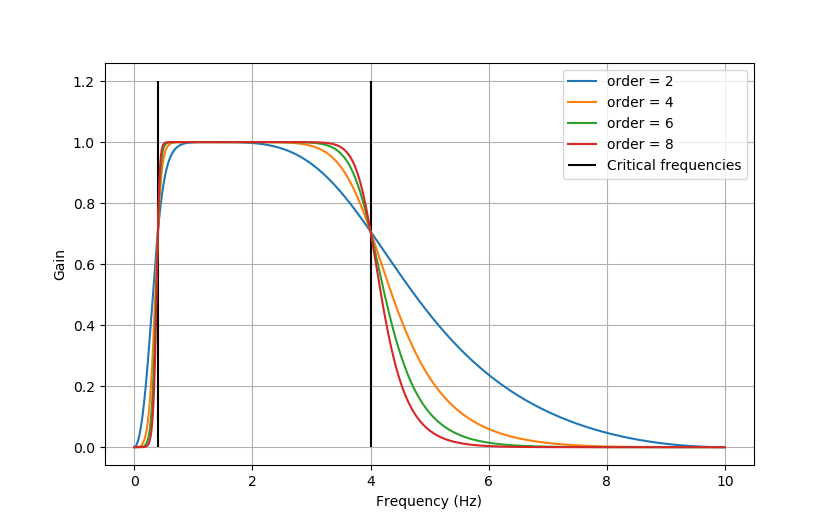
\includegraphics[width=0.8\textwidth]{figs/butter-order-comparison.png}}
\caption{Comparison of Butterworth filter orders}
\label{fig:butterworth-order}
\end{figure}

Order (\(N\)) controls the transition width - the higher the order, the lower
the transition width. This is desirable - we want to keep the passband as
large as possible, and transition quickly to the stopband. However, it comes
at the cost of computation complexity, as higher order filters take longer to
apply. See figure \ref{fig:butterworth-order} for a plot displaying the effect
of different orders on a filter's response.

Critical frequency gives the frequency at which we want gain to drop below
\(1/\sqrt2\) from the passband. Hence we use this parameter to define the
point from which we wish to cut out noise. Figure \ref{fig:butterworth-order}
uses critical frequencies 0.4 and 4 hz, which correspond to 24 and 240 bpm, a
reasonable heart rate range.

\subsection{Chebyshev Filter}

The Chebyshev filter aims to reduce the transition width as much as possible,
but to do this it introduces increased ripple.

\begin{figure}[h]
\begin{subfigure}{.5\textwidth}
  \centering
  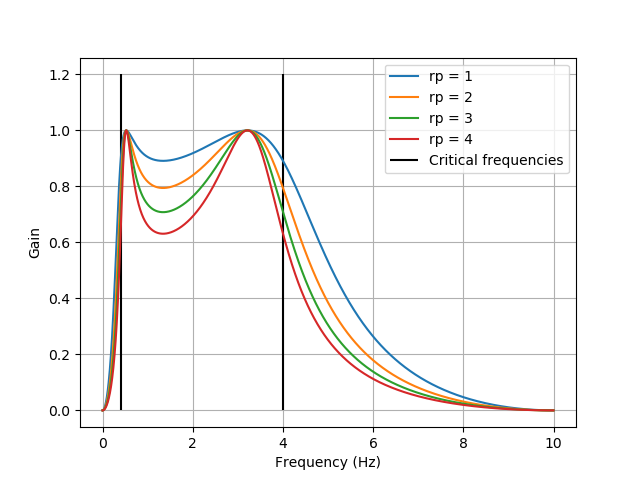
\includegraphics[width=\linewidth]{figs/cheby1-rp-comparison.png}
  \caption{Chebyshev Type 1}
  \label{fig:cheby1rs}
\end{subfigure}%
\begin{subfigure}{.5\textwidth}
  \centering
  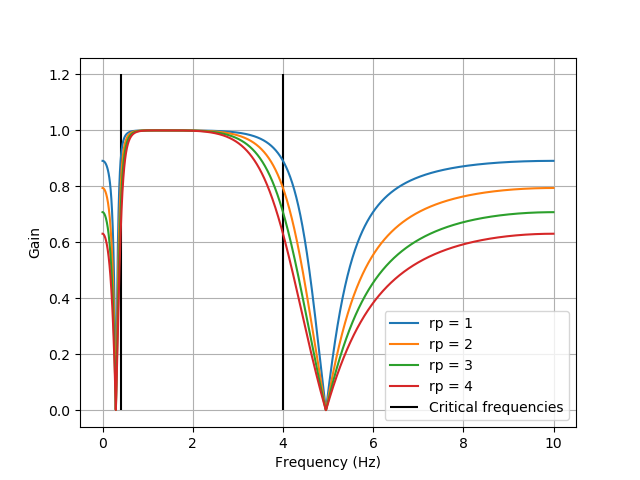
\includegraphics[width=\linewidth]{figs/cheby2-rp-comparison.png}
  \caption{Chebyshev Type 2}
  \label{fig:cheby2rs}
\end{subfigure}
\caption{Comparison of Chebyshev filter rp values}
\label{fig:chebyrp}
\end{figure}

The filter is defined with similar parameters to a Butterworth filter - order,
critical frequencies, and type all have very similar meanings. However,
there are type 1 and 2 Chebyshev filters, with different aims. Additionally,
there is a new parameter \emph{rp}. I will explain these differences here.

Type 1 Chebyshev filters introduce passband ripple, whereas type 2 Chebyshev 
filters introduce stopband ripple. Figure \ref{fig:chebyrp} shows how these
differences manifest in the response of a second order Chebyshev filter.

The parameter \emph{rp} is defined as the maximum ripple permitted below unity
gain. Higher \(rp\) results in more ripple for a type 1 filter, but less
ripple for a part 2 filter, as is demonstrated in figure \ref{fig:chebyrp}.
Introducing more ripple is undesirable as leads to more signal distortion,
however can be advantageous as it reduces the transition width.

\section{Motion Artefact Reduction}

In this section I explore a method which can be used to reduce the effect of 
Motion Artefacts (MAs) in the PPG Signal.

\subsection{Adaptive Noise Cancellation}

Adaptive Noise Cancellation (ANC), as described by Widrow et al.
\cite{Widrow75}, is a technique which allows us to remove noise from a signal,
given we have another signal correlated to the noise in some way. In our 
situation, we know MAs are correlated to motion, so we can use the 
accelerometer to remove MAs. This technique is extremely useful, as it can 
still produce good results when the MAs are at the same frequency as the heart
beat, even if the MAs have a larger amplitude.

%TODO: https://ieeexplore.ieee.org/abstract/document/7867772 this may be
%helpful


\begin{figure}[tbh]
	\centerline{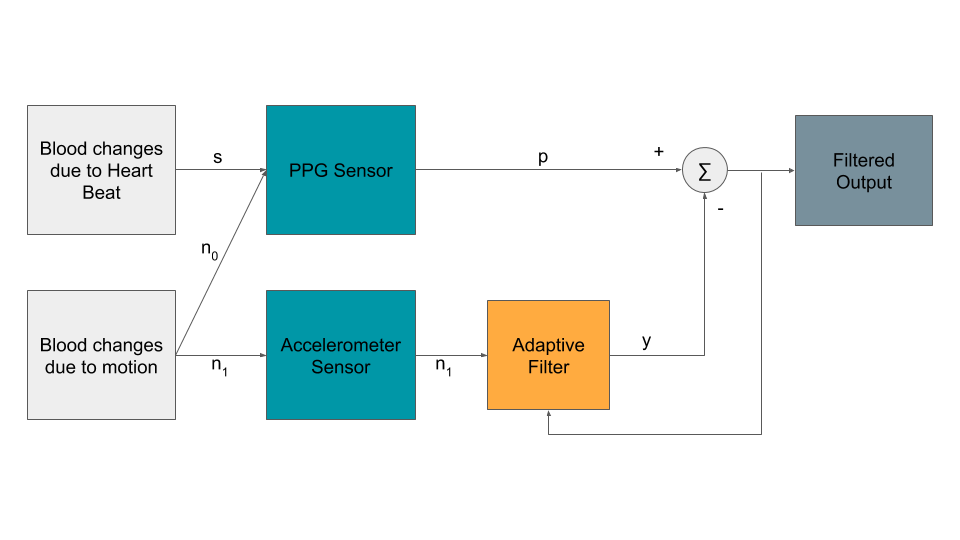
\includegraphics[width=\textwidth]{figs/ANC-concept.png}}
\caption{ANC overall flow}
\label{epsfig}
\end{figure}


An overview of the algorithm follows. We have signal from heartbeat \(s\) that
we want to figure out, but this is contaminated by noise from MAs \(n_0\).
We assume the PPG sensor reading \(p\) is such that \(p=s+n_0\). Additionally,
we have accelerometer sensor readings \(n_1\). We filter \(n_1\), producing
signal \(y\) and subtract this from \(p\), to produce \(z=p-y\). Our aim is to
adjust the filter, such that \(y\) is as close to \(n_0\) as possible. 

The type of filter we adjust is known as a Finite Impulse Response (FIR)
filter. An \(N\)th order filter is defined by \(N\) weights.
These weights are convolved with the signal, hence filtering it.

The adaptive filter aims to choose a filter such that the power of the output 
\(E[z^2]\) is minimized. Given \(s\) is uncorrelated with \(n_0\) and \(n_1\), and \(n_0\)
is correlated with \(n_1\), it can be proven that minimizing the output power
is equivalent to finding \(z=s\).

There are multiple algorithms which exist in order to adaptively filter a
signal. I'll look at two, first describing the least mean squares (LMS) algorithm from
Widrow and Hoff. LMS first initializes all of the filter weights to 0. At each
step, it finds the gradient of the mean square output \(E(z^2)\).
Each weight's gradient describes what would happen to the signal if we kept
using that weight value. So if the gradient of a weight is positive we know
that using that weight again would increase the mean squared output. Hence, at
the end of each step we shift the weights down if the gradient is positive,
and visa versa if the gradient is negative.

LMS takes a parameter - step size \(\mu\), which scales how much we move the
weights by. The equation used to update weights is \[w_{n+1}=w_n-\mu \nabla
E(y^2)[n]\]
where \(w_n\) is the \(n\)th filter weight, and \(\nabla E(y^2)[n]\) is the
\(n\)th weight gradient.

The LMS code I produced is as follows:

\begin{lstlisting}[language=Python]
def lms_filter(ppg, accel, K=15, step=1):
  """
  Run a least mean squares adaptive filter to remove noise from the signal
  that we know is correlation to the reference signal.

  Parameters
  ------------
   - ppg - the signal we want to remove noise from
   - accel - a signal we think is correlated with the noise
   - K - number of taps to use in the filter
   - step - step size to use

  Returns
  ------------
   - filtered - the signal with noise removed
  """

  N = ppg.size          # Size of PPG signal

  # Preprocessing
  freq = ppg.getFrequency()
  accel = accel.resample(freq)
  accel = accel.crop(N)

  accel = accel.getValues()
  ppg = ppg.getValues()

  w = np.zeros(K)      # Initial filter
  e = np.zeros(N-K)    # Initial error

  for n in range(0, N-K):
    accel_n = accel[n+K:n:-1]
    e_n = ppg[n+K] - np.dot(accel_n, w)          
    w = w + step * e_n * accel_n

    e[n] = e_n

  return data.getSignal(e_n, freq)
\end{lstlisting}

Step size must be chosen very carefully, as if it is too large there is a risk
of LMS missing the solution as it overcompensates for the gradient. If it is
too small, then the algorithm becomes too slow as we need many more
iterations. The situation is made worse as the ideal step size changes with
respect to the power of the input, making it very difficult to choose a step
size which gives stability.

To solve these stability issues, NLMS was introduced. It is the same as LMS, 
except you normalize the input power each
iteration. This makes choosing a step size which gives stability a lot easier.
The for loop from LMS above now looks like this:

\begin{lstlisting}[language=Python]
for n in range(0, N-K):
	accel_n = accel[n+K:n:-1]
	e_n = ppg[n+K] - np.dot(accel_n, w)          

	norm_factor = 1 / (np.dot(accel_n, accel_n) + 0.001)
	w = w + step * e_n * accel_n * norm_factor

	e[n] = e_n
\end{lstlisting}

So now we have a stable adaptive filter, which will allow us to tune a filter
that will remove motion noise from our PPG signal.

\section{Heart Rate Calculation}

Now we have removed noise from the signal, we should have a signal 
representing the volume of blood in veins within the arm. As the heart beats,
it sends a wave of blood through the body, forcing more blood through these
veins. Hence, peaks in the PPG signal correspond to heart beats. 

There are multiple approaches to finding heart-rate from our filtered
signals, and I will detail a few here.

\subsection{Local Maxima}

If we can find the peaks in the signal, we can count them up and divide by the
time period we count those peaks within, giving us a heart rate. One way we
can define peaks is as local maxima.

The local maxima in a signal are defined as samples (or successive samples of
the same amplitude) which are larger than both
neighbouring samples. In the case where we have multiple samples of the same
amplitude, the middle
sample position is returned (rounded down if necessary).
Finding local maxima is an easy problem to solve - 
intuitively, we can create an algorithm which iterates through the samples,
comparing each sample to its neighbours, which has complexity \(O(n)\).

\subsection{Peak-Peak Standard Deviation Minimization}
\label{sec:sd-min}

Finding the local maxima is a naive approach that doesn't adapt to any problem
specific knowledge. For example, we know heart-rate will not climb above 220
bpm, however the prior solution could report 300 bpm. Additionally, it might
find multiple local peaks around a single heart-beat. 

Ideally, we want to include knowledge about what a normal heart-beat looks
like in our detection algorithm. One thing we can do is look at peak-peak
intervals - the time that passes between heart beats. Surprisingly, this is
normally not consistent - a healthy heart actually beats with some
variation. However, when running it has been found that the heart beats with
very little variation \cite{michael17}, and hence in our case we can assume that the heart
beats regularly. The aim of this method is to use this assumption, along with
minimum and maximum heart-rate to better detect heart-beats.

The method begins by by calculating the
threshold, initially set as the rolling mean of the signal. It calculates a
set of initial peak
positions by finding positions where our signal crosses the threshold.
Then, it computes the standard deviation of the time between these peaks (peak-peak
intervals). Next, it iteratively increases the threshold and again calculates
the peaks, along with
the standard deviation of their intervals. The idea is every time it increases
the threshold we 
exclude more peaks. Then at the end, the peaks it actually selects are the peaks which give 
a reasonable
heart-rate (in the range 20-240 bpm), and have the smallest standard deviation.

The code I produced to do this is below:
\begin{lstlisting}[language=Python]
percs = [0, 5, 10, 15, 20, 25, 30, 40, 50, 60, 70, 80, 90, 100, 110, 120, 150, 200, 300]
mov_ave = moving_average(signal, window_size)
mov_ave = mov_ave.getValues()
signal_vals = signal.getValues()

min_sd = np.inf
current_peaks = []

for perc in percs:
    threshold = mov_ave + mov_ave * perc / 100

    #Find points above current moving average 
    x_peaks = (signal_vals > threshold).nonzero()[0]
    y_peaks = signal_vals[x_peaks]
    peak_edges = (np.diff(x_peaks) > 1).nonzero()[0] + 1

    # find the maximum between the peak edges. 
    peaks = []
    for i in range(len(peak_edges) - 1):
        ys = y_peaks[peak_edges[i]:peak_edges[i+1]].tolist()
        if len(ys) > 0:
            peaks.append(x_peaks[peak_edges[i] + ys.index(max(ys))])

    # Calculate standard deviation of the peak peak intervals
    intervals = np.diff(peaks) / signal.getFrequency()
    sd = np.std(intervals)

    if sd < min_sd and check_valid_hr(signal, peaks):
        min_sd = sd
        current_peaks = peaks

return np.array(current_peaks)
\end{lstlisting}

\section{Joint Sparse Spectrum Reconstruction}
\label{sec:joss}

So far all techniques I used to calculate heart-rate have worked in the time
domain, so now I'll look at using the frequency domain. I developed a
technique based on JOSS \cite{Zhang15.2}, which I discussed in the Section
\ref{joss-intro}. The algorithm is composed of two main stages, joint sparse
spectrum reconstruction and spectral peak tracking. 

\subsection{Joint Sparse Spectrum Reconstruction}

Joint sparse spectrum reconstruction is a method to estimate the spectrums of
multichannel signals. The problem can be summarised as solving the equation 
$$ Y = \Phi X + V $$

Where $Y \in \mathbb{R}^{M \times 4}$ is the matrix which has columns consisting of measurement vectors -
the first column contains $M$ PPG samples, and the second third and forth contain
the x, y and z acceleration samples. Where $N$ is the wanted resolution of
the Fourier transform, $\Phi \in \mathbb{C}^{N \times M}$ is the redundant discrete Fourier
transform basis matrix, as follows:
$$ \Phi_{m,n} = e^{i \frac{2 \pi}{N}mn},\ m = 0,\ldots,M-1;\ n=0,\ldots,N-1
\quad $$

$V \in \mathbb{R} ^{M \times 4}$ models noise, and $X \in
\mathbb{C}^{N \times 4}$ is the desired solution matrix. There are multiple
solutions for $X$, finding one is equivalent to finding the spectrum of each
of the input signals.

To calculate $X$, I make use of the MFOCUSS algorithm \cite{Cotter05}.
MFOCUSS is designed to solve undetermined systems of measurement vectors, such
as what we have. It is optimised to provide solutions where $X$ is sparse.
I used the
algorithm provided by Zhang \cite{ZhangCodes}, written in MATLAB, so I made use of the MATLAB
Engine API for Python in order to call the algorithm from my existing code. The 
following code shows my SSR function:

\begin{lstlisting}[language=Python]
def ssr(y, freq, N, eng):
    """
    Run sparse spectrum reconstruction using y sampled 
    at frequency freq, and a Fourier matrix to produce N 
    frequency taps. eng is the MATLAB engine used
    to run the MFOCUSS algorithm.
    """
    M = np.max(y.shape)

    # Make the Fourier matrix
    phi = np.zeros((M, N), dtype=complex)
    complex_factor = 1j * 2 * np.pi / N 
    for m in range(0, M): 
        for n in range(0, N): 
            phi[m,n] = np.exp(complex_factor * m * n)

    Phi = matlab.double(phi.tolist(), is_complex=True)
    Y = matlab.double(y.tolist())

    X = eng.MFOCUSS(Phi, Y, 1e-10, 'MAX_ITERS', 4)
    x = np.array(X)
    x = np.abs(x) ** 2


    return x
\end{lstlisting}

Now we have calculated the spectrums of the PPG signal and the noise, we can
remove noise from the signal, which is much easier in the frequency domain -
we simply subtract the spectrum of the motion noise from the spectrum of the
PPG noise, in order to reconstruct a clean spectrum. The advantage of using
the MFOCUSS algorithm and calculating the spectrums together is that the
frequency bins are much more likely to overlap between the accelerometer and
the PPG, where there is motion noise. 

The paper which describes JOSS \cite{Zhang15.2} recommends, for each frequency in the spectrum,
subtracting the maximum of all the accelerometer frequency bins from the PPG's
frequency bin. Additionally, it recommends setting all frequency bins below 
the maximum frequency bin divided by four to zero, in order to sparsify the array.
This is the relevant code:

\begin{lstlisting}[language=Python]
aggression = 0.99
accel_max = np.zeros((N))
signal_ssr = spectra[:,0]

# Modify the SSR signal by subtracting the maximum acceleration in each bin
for i in range(0, bpm.size):
    # Max of acceleration at this frequency
    accel_max[i] = np.max([spectra[i,1], spectra[i,2], spectra[i,3]])
    signal_ssr[i] = signal_ssr[i] - aggression * accel_max[i]

# Set all SSR bins lower than the maximum divided by 5 to 0
max_bin = np.max(signal_ssr)
signal_ssr[signal_ssr < max_bin / 4] = 0
\end{lstlisting}

So, now we have produced a spectrum of the PPG signal, with motion noise
removed, by computing the spectrums simultaneously.

\subsection{Spectral Peak Tracking}

We now have a spectrum, so we need some way of calculating heart-rate from it.
We could just select the largest peak in the spectrum, however this would be
naive - some noise may not be removed, so we could get random peaks.
Additionally, we know that heart-rate is relatively consistent so we can use
the previous heart-rate calculation to estimate the next one. Spectral peak
tracking helps to achieve this.

My spectral peak tracking initializes the heart-rate by looking for the
largest peak, as there will be little noise when the recording starts. Then,
it tries to find peaks, first peaks that are less than 15bpm away, then peaks
less than 25 bpm away. If no peaks are found, then the previously reported
heart-rate is used again as the heart-rate is likely lost in noise. If there
are multiple peaks, the algorithm takes the largest.

To avoid the heart-rate getting stuck at one value, a validation step is
included. If the bpm reported is the same for more than 3 successive
iterations, then
validation is triggered. To validate, we return the closest peak to the latest
recorded run, the code that finds this is below:

\begin{lstlisting}[language=Python]
def joss_spt(spectrum, freq, prev_loc, prev_bpm, trap_count):
    """
    Run spectral peak tracking

    Parameters
    ----------
     - spectrum : the spectrum of the signal
     - freq : sampling frequency
     - prev_loc : previous index of heart-rate bpm
     - prev_bpm : previous bpm calculated
     - trap_count : number of times bpm has been the same

    Returns
    ----------
     - loc : location of bpm calculated
     - bpm : bpm calculated
     - trap_count : number of times bpm has been the same

    """
    deltas = [15, 25]

    N = spectrum.size

    # If initialising
    if prev_loc == -1 and prev_bpm == -1:
        loc = np.argmax(spectrum)
        bpm = 60 * loc / N * freq

    else:
        for delta in deltas:
            rng = np.arange(prev_loc - delta, prev_loc + delta)

            # find peaks in range
            mask = np.zeros((N,))
            mask[rng[rng>0]] = 1
            filtered = (spectrum * mask).flatten()
            locs, _ = scipy.signal.find_peaks(filtered)
            vals = filtered[locs]

            num_peaks = locs.size
            if num_peaks > 0:
                max_index = np.argmax(vals)
                loc = locs[max_index]
                bpm = 60 * loc / N * freq
                break

        else:
            loc = prev_loc
            bpm = prev_bpm

    # validate results
    if loc == prev_loc:
        trap_count += 1
        if trap_count > 10:
            loc = discover_peak(spectrum, prev_loc)
            bpm = 60 * loc / N * freq

    else:
        trap_count = 0

    return loc, bpm, trap_count


def discover_peak(spectrum, prev_loc):
    """
    Find the closest peak in spectrum to the peak at prev_loc.
    """
    rng = np.arange(40, 220)
    N = spectrum.shape[0]

    # find peaks in range
    mask = np.zeros((N,))
    mask[rng] = 1
    filtered = (spectrum * mask).flatten()
    locs, _ = scipy.signal.find_peaks(filtered)

    if locs.size == 0:
        return prev_loc

    # find closest peak to prev_loc
    dist = np.abs(prev_loc - locs)
    index = np.argmin(dist)
    loc = locs[index]

    return loc
\end{lstlisting}

Now, we have developed another method to calculate heart-rate which
removes MAs in the frequency domain and uses previous data to better calculate
current heart-rate.

\section{Earbuds}

As an extension, I wanted to collect heart-rate from earbuds containing PPG
sensors. In theory, they 
are less affected by motion noise
because they are not influenced by arm movement. Additionally, the ear has a rich set
of veins which is perfect for PPG analysis. For the purposes of this project I used
a set of Jabra elite sport earbuds, which have a PPG sensor under the right
bud - see figure \ref{fig:jabra}. 

Unlike with the watch, there is no way to extract the raw PPG signal from the
earbuds, so I have to work with the derived heart-rate signal, as provided by
their algorithms. 

My watch is able to connect to the earbuds using Bluetooth, so I connect them
and
the following details the process of collecting data from the earbuds. 

\begin{figure}[tbh]
	\centerline{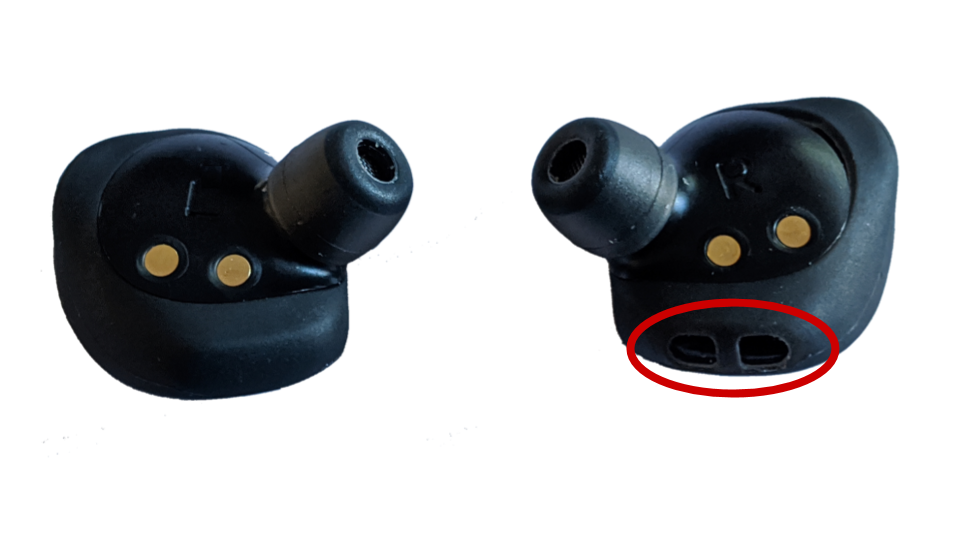
\includegraphics[width=0.4\textwidth]{figs/jabra.png}}
	\caption{Positioning of the PPG sensor on Jabra elite sport earbuds.}
	\label{fig:jabra}
\end{figure}

\subsection{Gathering data}

To collect data, I connected the earbuds to the watch, and then data is
sent through the Bluetooth Light Energy (LE) protocol. There are a few key
pieces of terminology, which I explain here:

\paragraph{Generic Attribute Profile (GATT)} describes the overall methods
with which data values are transported by Bluetooth LE.

\paragraph{GATT Server} is a device which stores and distributes information. In
our case the earbuds are a GATT server.

\paragraph{GATT Client} is a device which requests information from a GATT
server, in our case a smart watch.

\paragraph{Characteristics} are single data points, for example in our case a
heart-rate integer. Characteristics also have a number of descriptors
describing the value.

\paragraph{Services} are logical group of characteristics, for example the
heart-rate service contains the heart-rate measurement characteristic along
with sensor position characteristic.

\paragraph{Characteristic Value Notifications} are sent from client to server
to indicate that the client would like to receive updates when a certain
characteristic is changed. This is how frequently changing values are passed
over Bluetooth LE, as it is more power efficient than having the client
periodically request updates.
\\
\\

Figure \ref{fig:gatt-flow} shows the flow I aimed to introduce in my data collection program to run
on the watch. In Kotlin, I iterate through the connected Bluetooth devices,
until I find the earbuds, and then the app connects to the earbud's GATT
server. Once connected 
to the GATT server, the app
requests notifications for the heart-rate characteristic. These
characteristics are then periodically sent to the watch, where they are
recorded.

\begin{figure}[H]
	\centerline{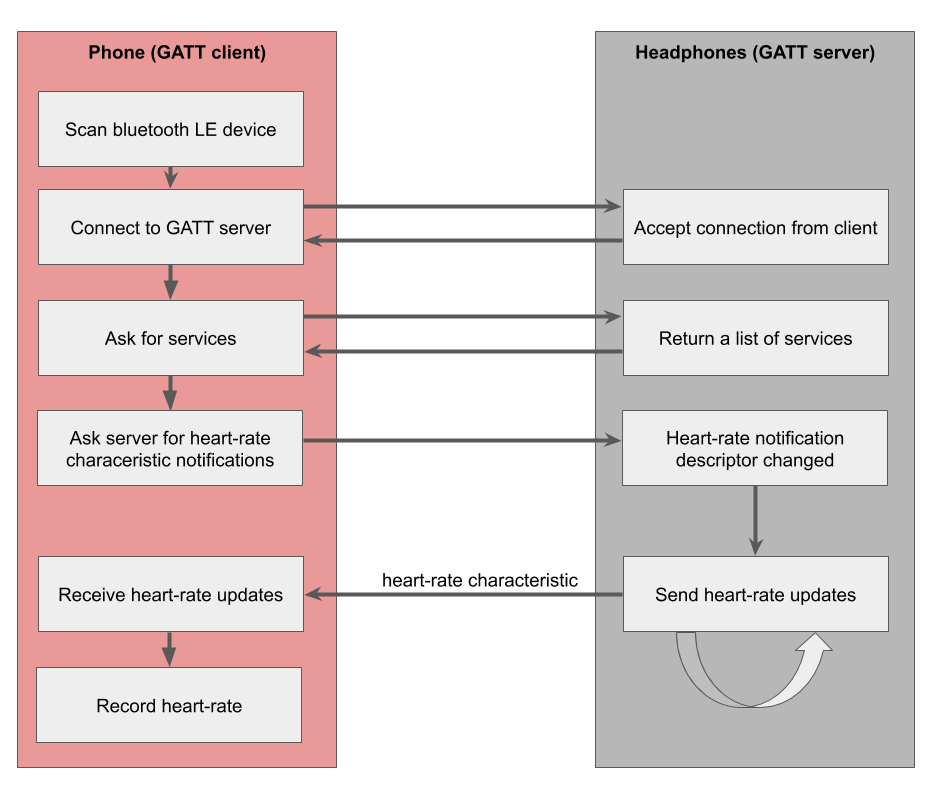
\includegraphics[width=0.7\textwidth]{figs/gatt-flow.png}}
	\caption{Retrieving Data from Earbuds.}
	\label{fig:gatt-flow}
\end{figure}

\subsubsection{Android Services}

In order to avoid the data being lost when the application leaves the screen,
I implemented all of the Bluetooth functionality within a service. A service
allows code to run when the application isn't in focus. It does add some
complexity into development though, as I describe here.

When a service is created, it is bound to the application which starts it.
When a service is bound, the application can send requests, and receive
updates from it - as I'll discuss further on. However, when an application is
out of focus, services bound to it are destroyed, and hence our service must
be unbound before this happens. Then, when our application comes back into
focus, we rebind it, see the code below:

\begin{lstlisting}[language=Kotlin]
override fun onStart() {
    // Bind the service.
    Intent(this, HeartDeviceService::class.java).also { intent ->
        bindService(intent, mServiceConnection, Context.BIND_AUTO_CREATE)
    }
    super.onStart()
}

override fun onStop() {
    unbindService(mServiceConnection)
    super.onStop()
}
\end{lstlisting}

In order to receive updates from the service, we must use intents, which are
the way Android allows different applications to communicate. 
We create a \emph{BroadcastReceiver}
object in \emph{MainActivity}, which deals with intents we might receive from
the service - the intents it may send include device connected/disconnected
and an update to say the recordings have successfully been saved. 

\begin{lstlisting}[language=Kotlin]
// Handles various events fired by the Service.
// ACTION_GATT_CONNECTED: connected to a GATT server.
// ACTION_GATT_DISCONNECTED: disconnected from a GATT server.
// ACTION_SAVED: heart-rate data has been saved
private val mGattUpdateReceiver = object : BroadcastReceiver() {
    override fun onReceive(context: Context, intent: Intent) {
        val action = intent.action
        when {
            HeartDeviceService.ACTION_GATT_CONNECTED.equals(action) -> {
                mConnected = true
                showConnected(mConnected)
            }
            HeartDeviceService.ACTION_GATT_DISCONNECTED.equals(action) -> {
                mConnected = false
                showConnected(mConnected)
            }
            HeartDeviceService.ACTION_SAVED.equals(action) -> {
                mRecordingStarted = false
                mSaveListener.onSave()
            }
        }
    }
}
\end{lstlisting}


\subsection{Sensor Fusion}

Once I had gathered data from the earbuds, I evaluated it and found a problem,
see section \ref{sec:earbud-problem} for details. In essence, the issue I
found was that the earbuds would lose the heartbeat signal due to the sensor
changing position during a run. Particularly annoyingly, the earbuds report a
heart-rate of zero whenever this happens. 

To rectify this, I will implement a sensor-fusion technique. This technique
makes use of a Kalman filter. The idea is it takes measurements from the earbuds, which
we know are accurate, and then in periods where the heart-beat signal drops
out we guide the output using the less accurate PPG from the wrist-watch.

\subsection{Kalman Filter}

A Kalman filter can be used to estimate the value of an unknown variable, by
producing a probability distribution for that variable that is updated over
time.
It consists of two phases:
\begin{enumerate}
	\item Prediction step - predict the current heart rate based on the
		previous heart-rate, and the readings from the watch PPG.

	\item Correct step - when we get a confirmed measurement from the
		earbuds, we move the heart-rate to the earbud's estimation.
\end{enumerate}

The Kalman filter relies on modelling current heart-rate as a Gaussian
distribution with its standard deviation representing the certainty of the
current estimate.

Kalman gain is the parameter used to weight the measurements against the
prediction. A higher gain assigns more trust to the measurements, meaning the
filter will respond quicker, a low gain produces more smoothing.

The code for my Kalman filter is as follows:


\begin{lstlisting}[language=Python]

def predict(self, t, old_hr, old_var):
    if t < 1:
        raise ValueError("Predict step must start at time t > 0")

    # calculate hr difference between t-1 and t on the watch
    diff = self.watch[t] - self.watch[t-1]

    hr = old_hr + diff
    var = old_var + self.predict_var

    return hr, var


def correct(self, t, predicted_hr, predicted_var):
    # Calculate Kalman gain
    k = predicted_var  / (predicted_var + self.ear_noise)

    # Calculate new hr and variance
    hr = predicted_hr + k * (self.ear[t] - predicted_hr)
    var = (1 - k) * predicted_var

    return hr, var


def filter(self):
    hrs = np.zeros(self.size)

    # Initial step, wait until we get some data from the ear sensor before starting the filter
    t_min = 1
    while self.ear[t_min] == 0:
        t_min += 1

    hr = self.ear[t_min]
    var = self.ear_noise

    # Run the Kalman filter
    for t in range(t_min, self.size):
        hr, var = self.predict(t, hr, var)

        if self.ear[t] != 0:
            hr, var = self.correct(t, hr, var)

        hrs[t] = hr

    return data.Signal(hrs, 1)

\end{lstlisting}

In this section I have developed an application which gets heart-rate data from
earbuds, and have implemented a Kalman filter which allows us to fuse the data
from the watch and earbud sensors, hopefully giving us more accurate results.


\section{Repository Overview}
Below is an overview of the structure of my project. A more detailed version
is given in Appendix \ref{app:repo_overview}.

{\scriptsize
\begin{forest}
  for tree={
    font=\ttfamily,
    text width=\textwidth,
    grow'=0,
    child anchor=west,
    parent anchor=south,
    anchor=west,
    calign=first,
    edge path={
     \noexpand\path [draw, \forestoption{edge}]
    (!u.south west) +(7.5pt,0) |- node[fill,inner sep=1.25pt] {} (.child anchor)\forestoption{edge label};
 },
    before typesetting nodes={
      if n=1
        {insert before={[,phantom]}}
        {}
    },
    fit=band,
    before computing xy={l=15pt},
  }
[
  [{\bf ppg-recorder/app/src} - Contains Android project designed for the
	  watch
	  [\emph{EarHRRecorder.kt} - Controls recording HR from bluetooth
	  earbuds]
	  [\emph{HeartDeviceService.kt} - The service which listens for
	  updates from Bluetooth updates in the background]
	  [\emph{MainActivity.kt} - Runs the main thread of the program]
	  [\emph{PpgRecorder.kt} - Records data from the watch's PPG sensor]
	  [\emph{Sync.kt} - Uploads recorded data to a server]
  ]
  [{\bf server} - A server to run on a raspberry pi and receive data
	  [\emph{gdrive.py} - Uploads files to Google Drive]
	  [\emph{server.py} - Server code built with Flask]
  ]
  [{\bf data} - Contains files to process the recordings in addition to the recorded data
    [{\bf evaluation} - Programs used to evaluate the project]
    [\emph{filtering.py} - Runs a butterworth and chebyshev filter]
    [\emph{joss.py} - Runs spectrum reconstruction on watch data]
    [\emph{kalmanfilter.py} - Implementation of Kalman filter]
    [\emph{motionfilter.py} - Implementation of LMS and NLMS]
    [\emph{peakfind.py} - Naive and sd-minimisation peakfinding functions]
    [\emph{sync.py} - Code which combines watch and ECG data ensuring they start at
    the same time]
  ]
]
\end{forest}
}


\chapter{Evaluation}

In this chapter, I describe the steps I took in order to evaluate both
functionality and performance of my project. I go through all the
implementation stages - gathering data, filtering data, motion artefact
reduction, heart-rate calculation, spectrum reconstruction and dealing with earbuds -
for each commenting on their accuracy and performance.

\section{Gathering Data}

\subsection{Synchronising Signals} \label{sec:evaluate-sync}

In section \ref{sec:sync}, I detailed an algorithm which allowed me to
calculate the difference in start-times between different recordings from a
watch and from an ECG. Initially I used cross-correlation of accelerometer signals to
determine the time at which the signals are the most similar, however this is
quite inefficient, so I also developed an improved algorithm, referred to as
informed cross correlation from now on.

In this section, I will evaluate both the validity and the performance of the
solutions. To prove validity of informed cross correlation, I compare the
time difference it predicts to the actual time difference calculated by cross
correlation, and then take the average absolute error over all recorded runs,
in seconds. 

To evaluate performance of informed cross correlation I run the
algorithm on a sample set of accelerometer data, 500 times, using the python
module timeit. This module avoids some easy mistakes that can be made when
measuring execution times in python, for example it uses
\emph{time.perf\_counter()} to measure time, which only measures execution
time, not time spent sleeping. I repeat 500 times so that the average is not
affected too much by other processes that might be running.

Informed cross correlation takes an additional parameter,
\emph{g} which describes how many seconds to skip whilst
calculating the initial cross correlation. I will test the algorithm with different
values of this parameter, so I can determine which gives the best performance
whilst still being valid. 

The results of my test are displayed in Table \ref{table:cross-correlation}. 

\begin{table}
\centering
\caption{Comparing Cross-Correlation Techniques.}
\label{table:cross-correlation}
\begin{tabular}{ | c | c | c | }
	\hline
	Algorithm & Average Absolute Error (s) & Time for 500
	iterations (s)\\ 
	\hline
	Cross correlation & 0 & 112.227 \\  
	Informed g = 0.1s & 0 & 17.935 \\    
	Informed g = 0.25s & 0 & 11.089 \\    
	Informed g = 0.5s & 0 & 8.648 \\    
	Informed g = 1s & 0.137 & 7.069  \\
	\hline
   \end{tabular}
\end{table}

The first result I draw from this table is that my informed algorithm leads to
a significant improvement in performance. Even the slowest informed runtime is 6
times faster than the naive implementation. Next, it can be seen that the
runtime of the informed algorithm increases as the size of g decreases. This
makes sense as the smaller the size of g, the fewer cross-correlation values
we calculate.

In terms of validity, the table shows that the total absolute error of the
informed algorithm is 0, for all values of \emph{g} up to \emph{g} = 1s. As
\emph{g} increases, the likelihood that the initial scan misses the optimal
solution increases because the step size is too large. 

In conclusion, I have discovered that the informed algorithm is capable of
giving a valid solution, although if the value of \emph{g} rises too high the
solution may no longer be valid. In addition, I have discovered that it gives
a much quicker solution, which gets quicker as \emph{g} rises. For safety, I
would choose \emph{g} = 0.25s, which ensures the result will be valid, whilst
still providing a ten-fold performance increase.


\section{Filtering}

To test filters, I will run two different tests. Firstly I will test how much
noise the filter can remove alongside how much the information we want is
actually retained. Additionally
I will test how the speed of the filters
varies, as we want the filter to run as quick as possible.

To test the quality of the filter I devised a test where I simulate a possible
PPG signal without noise, then add noise. The noise I add will be random
amount of high and low frequency noise, as we get in an actual PPG signal.
Then to calcualte the quality of the filter, I filter the signal, and compare
the power spectrums of the filtered signals to the clean signal.

To simulate PPG signals, I found that two Guassians could be used
\cite{Banerjee15}. One Gaussian represents the higher systolic peak, and the
other represents the lower diastolic peak. 
See figure \ref{fig:sim-beat} for an example of the clean signal my simulation
produces. As heart-rate is relatively
consistent during running, I can assume the peaks are in approximately the
same position, with slight variation. I simulate a heart-rate of 120 bpm, by
repeating the pattern heart-beat every 0.5 seconds. In each beat I randomly
vary the amplitude of both peaks, as would happen with an actual heart-beat.
See figure \ref{fig:sim-beats} for a simulated heart-beat of 5 beats.

To represent the noise, I add a random Gaussian noise to each sample, to
represent the measurement error, along with low frequency noise at 0.2 and 0.3
hz, representing the noise present for example due to temperature variation,
and breathing.  
The results of adding this noise to a signal can be seen in figure
\ref{fig:sim-beats-noise}.

\begin{figure}
	\centering
	\begin{subfigure}[b]{0.4\textwidth}
		\centerline{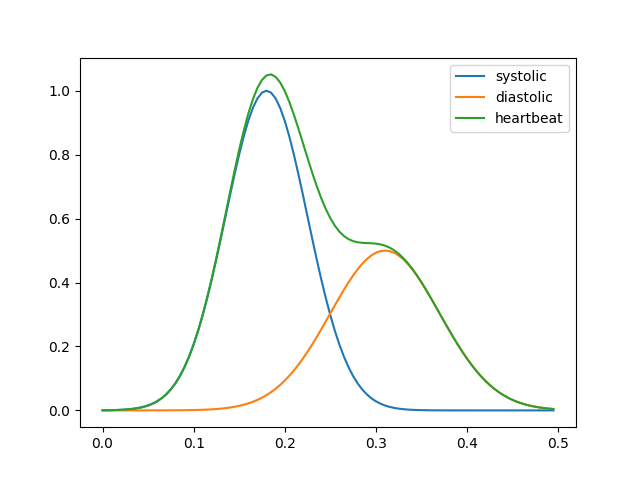
\includegraphics[width=\textwidth]{figs/sim-beat.png}}
		\caption{A single simulated beat.}
		\label{fig:sim-beat}
	\end{subfigure}
	\hfill
	\begin{subfigure}[b]{0.5\textwidth}
		\centerline{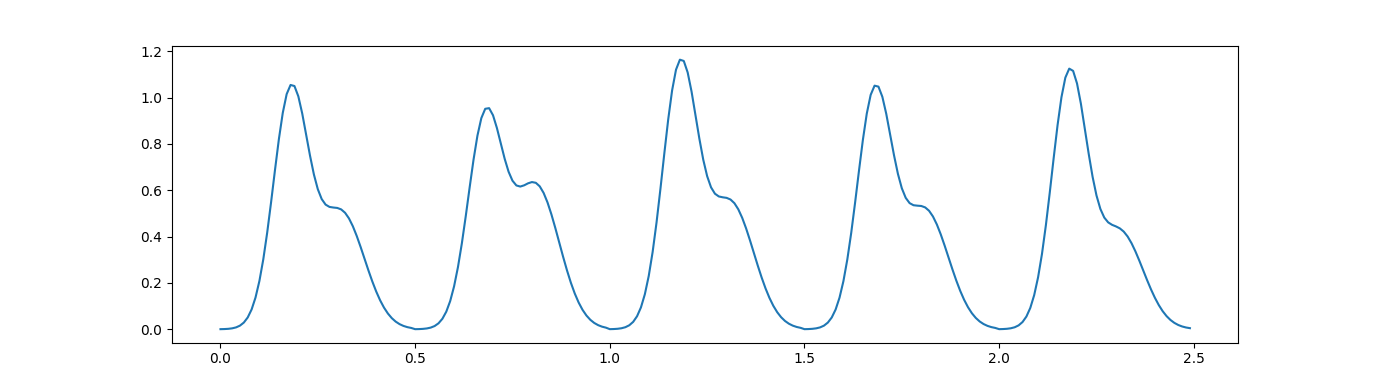
\includegraphics[width=\textwidth]{figs/sim-beats.png}}
		\caption{Multiple simulated heart-beats.}
		\label{fig:sim-beats}
	\end{subfigure}
	\hfill
	\begin{subfigure}[b]{0.6\textwidth}
		\centerline{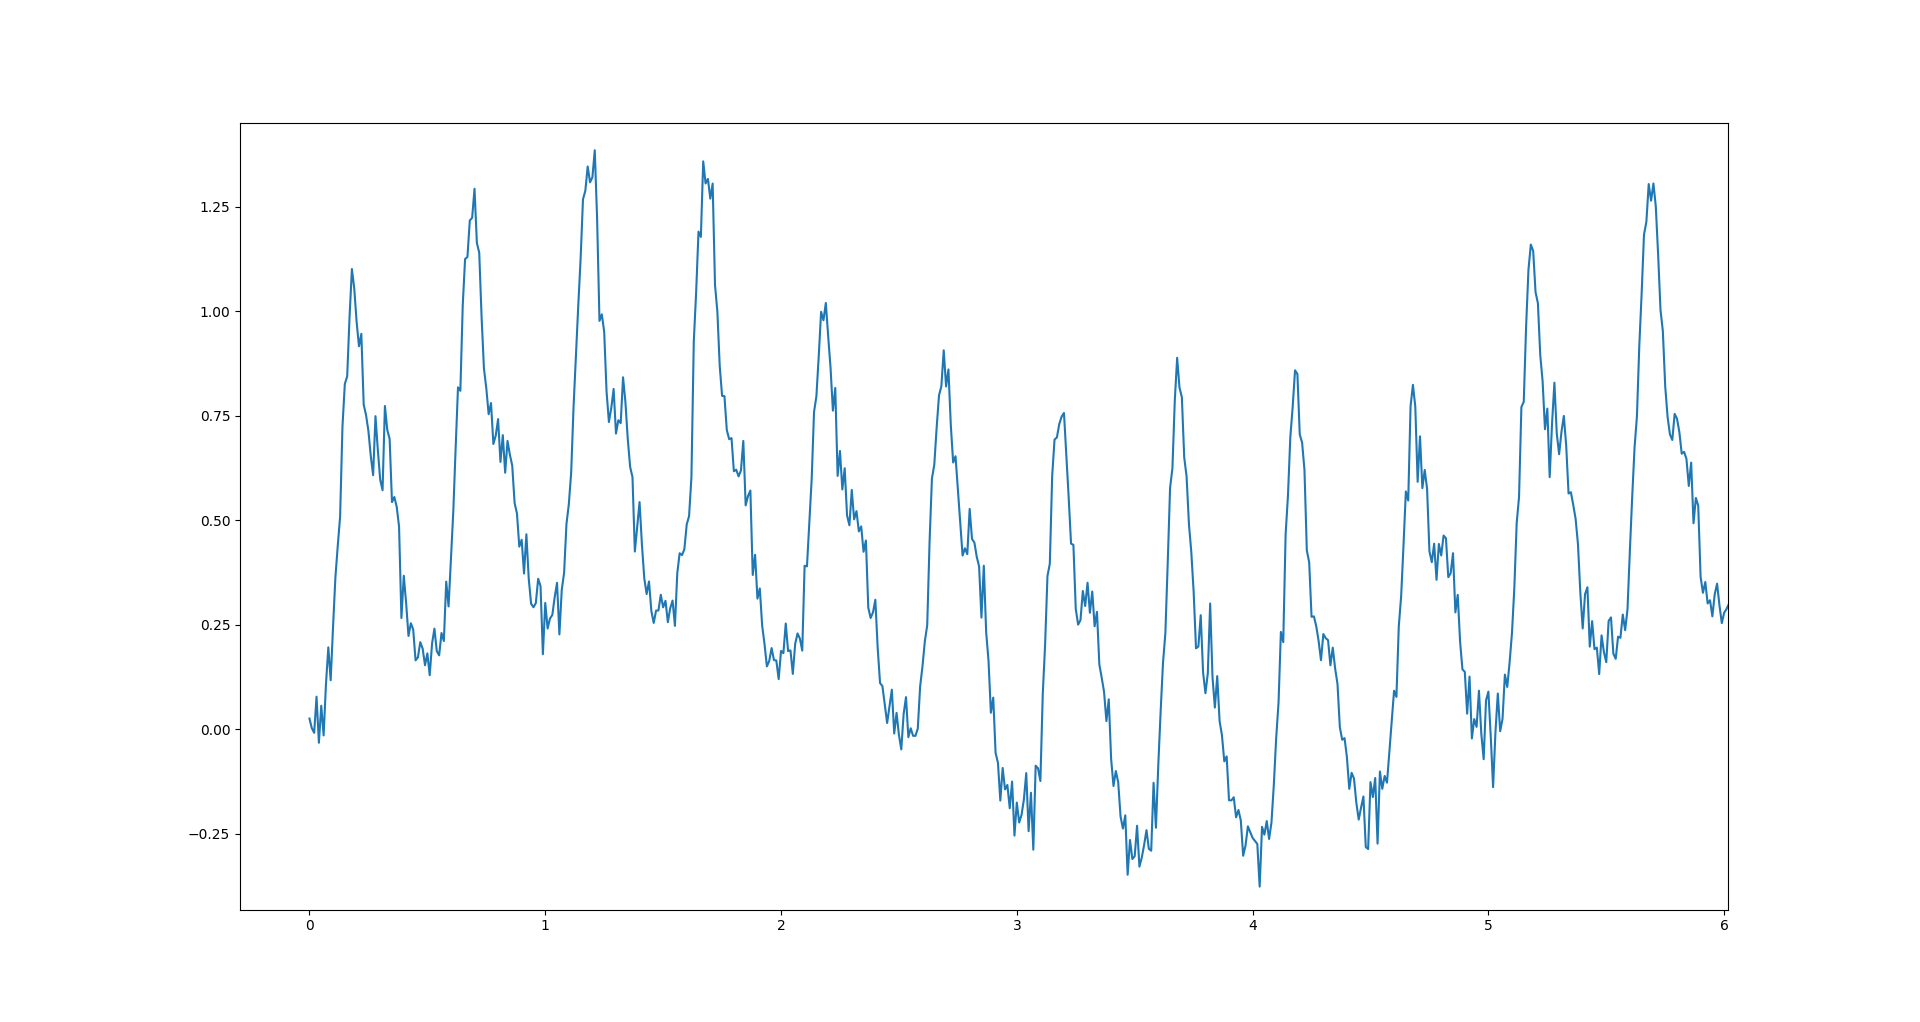
\includegraphics[width=\textwidth]{figs/sim-beats-with-noise.png}}
		\caption{Simulated heart-beats with noise.}
		\label{fig:sim-beats-noise}
	\end{subfigure}
	\caption{Simulating a noisy heart-beat.}
\end{figure}

Next, I must test the speed of the algorithms. To test this, I run the filter
on a sample run from which I have collected 10 minutes of data. I run the test
500 times and take an average over the time taken.

I test the Chebyshev filter and the Butterworth filter with different
parameters, in order to decide between the two of them, and additionally what
parameters are optimal, in terms of both speed and validity.

\subsection{Butterworth Filter}

I test the validity of the filter by comparing the power spectrum produced by
filtering the simulated heart-beat I detail above. The power spectrums are
shown in figure 
\ref{fig:butterworth-validity}. For reference, at the top of the figure we
plot the power spectrum of the clean signal and that signal with noise added.
Ideally, we are looking to see the clean signal spectrum once we have filtered the
noisy signal. The clean signal spectrum shows a clear peak at 2 hz, which
corresponds exactly to the heart-rate we chose - 120 bpm. Additionally, there
are peaks at 4 and 6 hz which are a feature of the power spectrum - it
produces peaks at 2, 3, 4, and so on times the principle frequency. The noisy
spectrum shows the additive Gaussian noise, which is present at every
frequency, and additionally a small peak at around 0.2 hz, which shows the low
frequency noise. I will compare how effective the filters are at removing both
the random noise and the low frequency noise.

The results show that at all orders, the desired signal at 2 hz is present.
However, as the filter order increases, the amount of random noise present
decreases. The 1st order filter has a wide range of random noise, whereas the
5th order filter removes almost all noise outside the range 0.4 to 4 hz. This
is as higher-order filters have a smaller transition between the passband and
stopband.
Interestingly, there is an artefact in the 6th order filter, where there is a
spike at 0.3 hz, which is larger than the desired signal, so I will avoid
using these. 

\begin{figure}
	\centering
	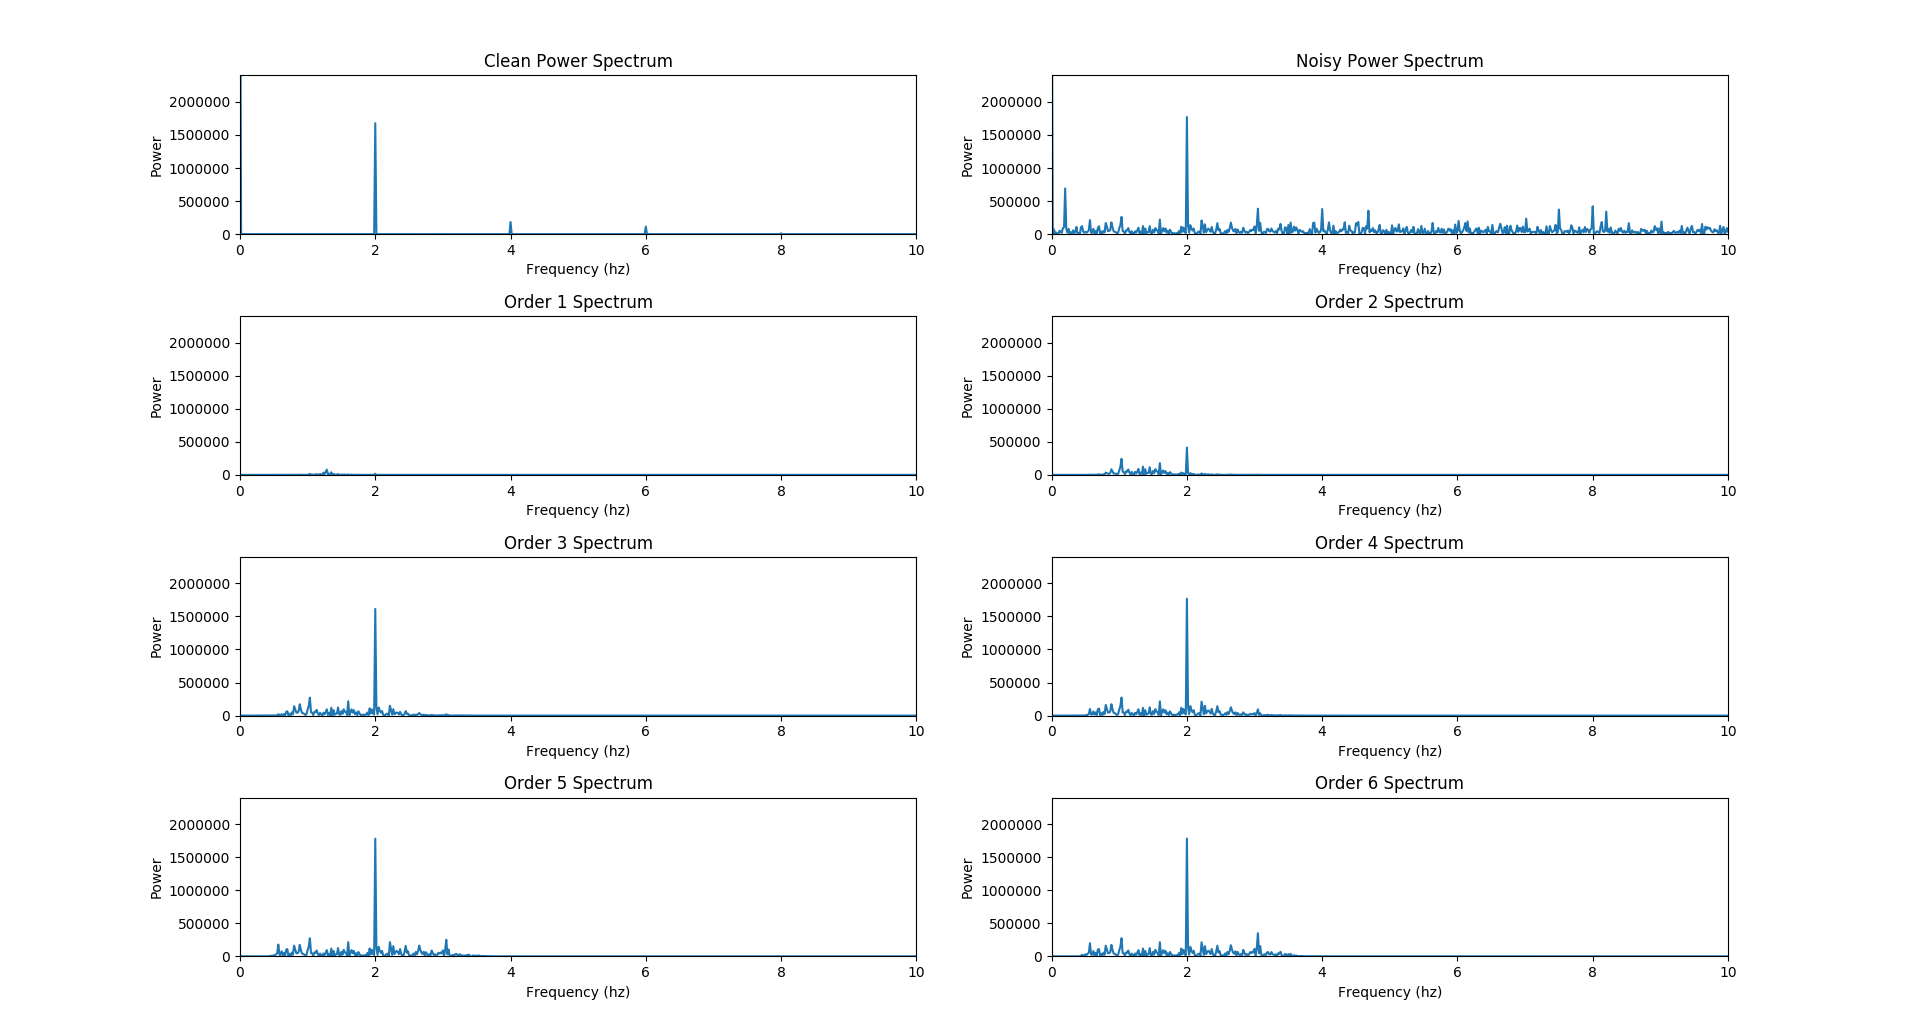
\includegraphics[width=\textwidth]{figs/butterworth-validity.png}
	\caption{Butterworth Filter Power Spectrums.}
	\label{fig:butterworth-validity}
\end{figure}


I test the speed by running the filter 1000 times (to remove the effect of
other processes) using python's
\emph{timeit.timeit()} function, which provides the accurate time the computer
has spent evaluating a given piece of code. I run the test on the same 35
minute PPG I recorded on a run. 

The results of the timing test can be seen in figure \ref{fig:butter-time}.
The graph shows that generally higher order results in greater
execution time, but the effect is not linear- there is a smaller increase
in execution time 
between an odd order and the next order. Timing is very important for our use
case, as in production the algorithms would run on the watch. The watch has
very limited power, so the less time the algorithm takes, the better.

If choosing a Butterworth filter, I would opt for a 5th order filter, as it
provides the most filtering, whilst not producing artefacts as seen in the 6th
order filter. 

\begin{figure}[tbh]
	\centerline{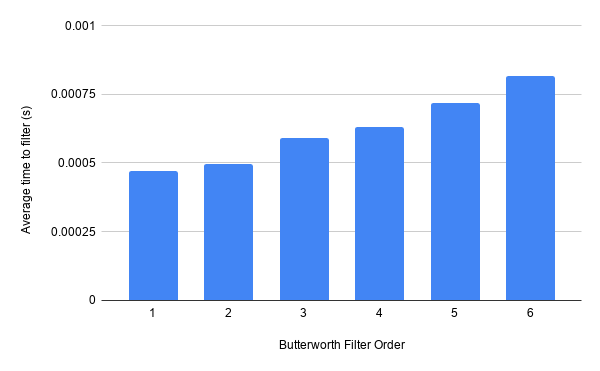
\includegraphics[width=0.5\textwidth]{figs/butter-time.png}}
	\caption{The effect of Butterworth filter order on execution time.}
	\label{fig:butter-time}
\end{figure}

\subsection{Chebyshev Type II Filter}

I test the validity of the filter by again comparing the power spectrum produced by
filtering the simulated heart-beat I detail above. The power spectrums are
shown in figure 
\ref{fig:cheby2-validity}. 

The results show that an order 1 filter is not useful, as there is almost no
useful signal present. This is as a first order Chebyshev Type-2 filter
provides a very narrow pass-band, resulting in almost no useful signal passing
through. The order 2 filter is an improvement, and there is a
clear peak at 2 hz, however it is about as powerful as the random noise,
meaning we have not recovered the signal as accurately as we might want. 
Orders 3,4,5 and 6 are all very
similar, with a very clear peak at 2 hz, and the random noise only present
between 0.4 and 4 hz, as we wanted from the filter. The 2 hz peak is also much
larger than the random noise, as desired. All of the filter orders effectively
dealt with the low frequency noise, it is not featured within the power
spectrums at all.


\begin{figure}
	\centering
	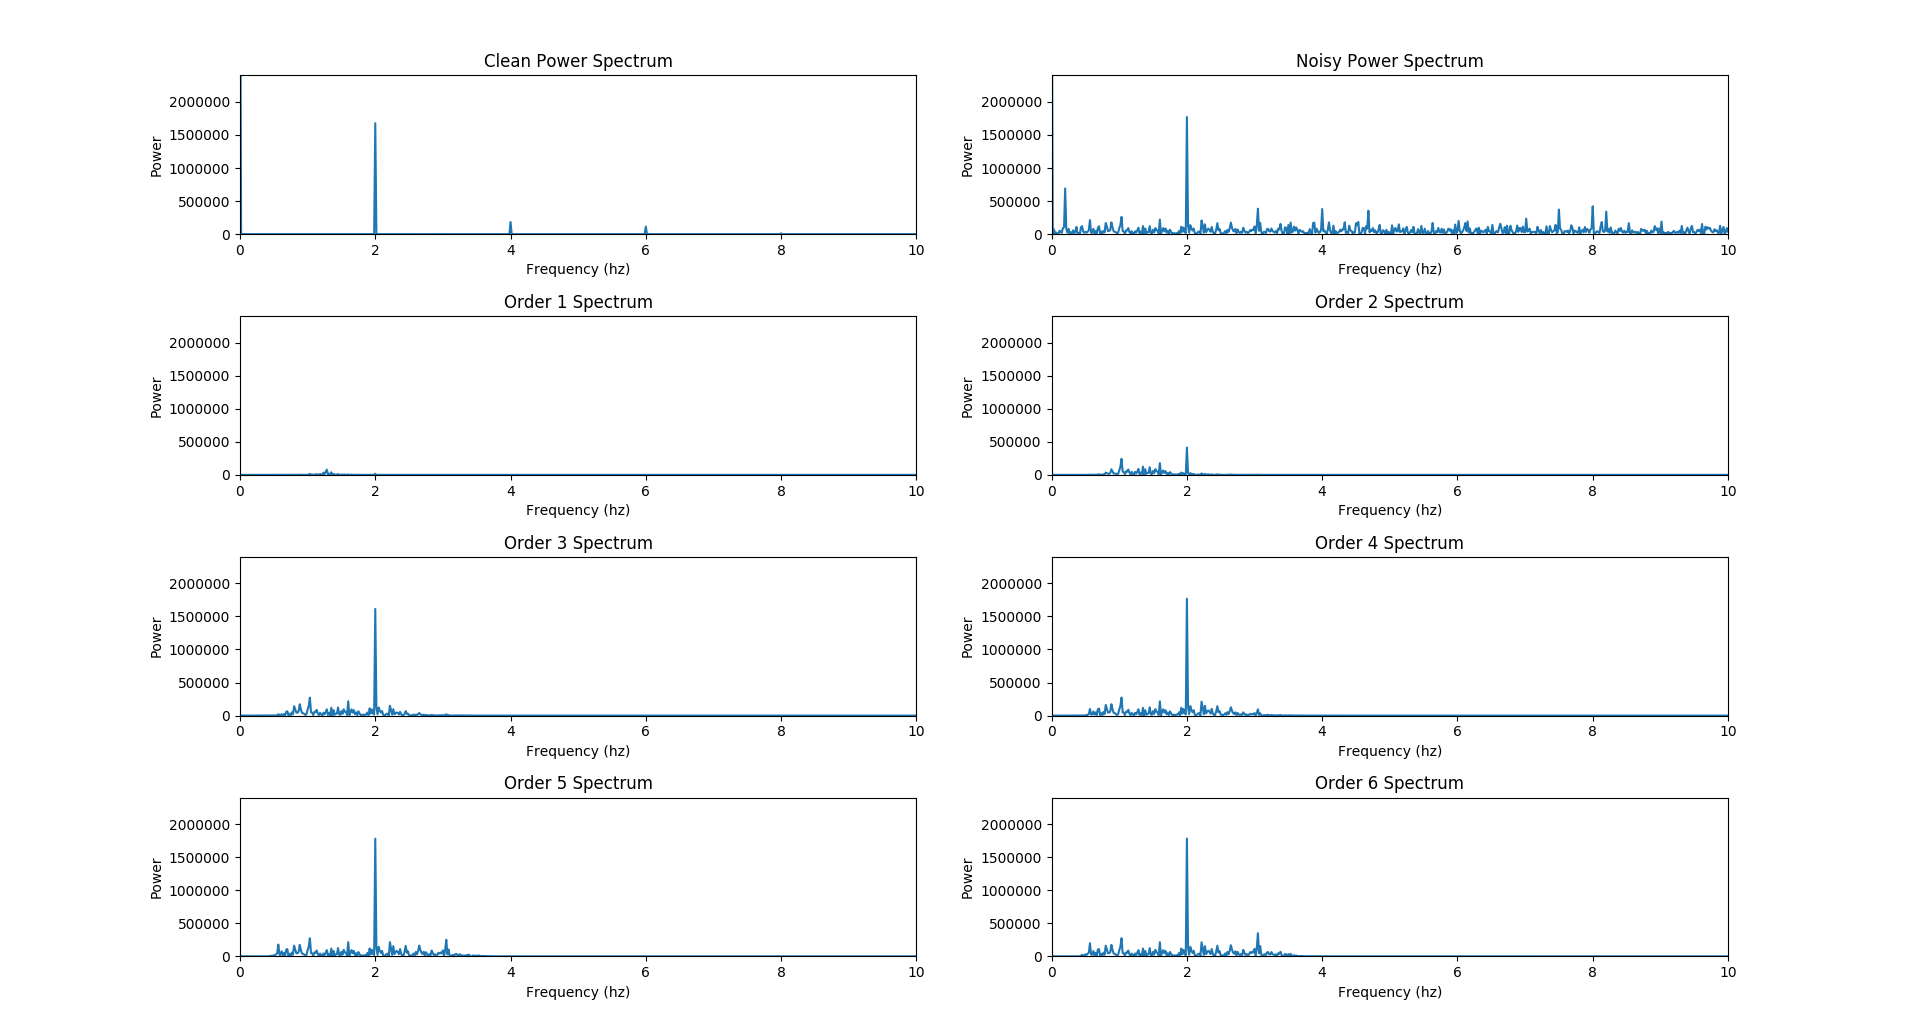
\includegraphics[width=\textwidth]{figs/cheby2-validity.png}
	\caption{Chebyshev Filter Power Spectrums.}
	\label{fig:cheby2-validity}
\end{figure}

I run the timing test again on the Chebyshev type II filter, taking the average amount
of time taken to filter the same 35 minute segment as before. The results are
plotted along with the Butterworth times in figure \ref{fig:cheby2-time}. 
Firstly, there is a clear linear
correlation between increasing filter order and increased execution time. This
implies we should choose the lowest filter order which is feasible. Secondly,
note that the Chebyshev filter takes over double the time as the
Butterworth filter for each order.

If I was going to choose a Chebyshev Type II filter, I would choose an order 3
filter, as it provides sufficient filtering, without reducing the power of the
useful signal too much. Additionally, any higher-order filters would take too
much time.

\begin{figure}[tbh]
	\centerline{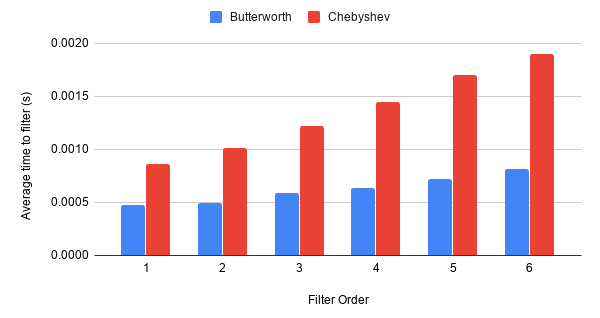
\includegraphics[width=0.5\textwidth]{figs/cheby2andbutter-time.png}}
	\caption{The effect of Chebyshev and Butterworth filter order on execution time.}
	\label{fig:cheby2-time}
\end{figure}


\section{Motion Artefact Reduction}

In this section I talk about the work done to evaluate the effectiveness of my
motion artefact reduction techniques. 
I first detail the tests I
ran, followed by the results of these tests on the different algorithms.

I will test the algorithms on different levels of motion corruption, to
determine what solution is most effective for each level. I divide the
data into twenty second segments of PPG data, labelled with the running speed. For
testing motion artefact reduction, I only test data recorded while running at
a speed greater than 3 km/h.

Now, to test my motion filtering algorithm, for each PPG data segment, I run
the algorithm on it. With the results, I calculate the heart-rate that my
heart-rate algorithm would compute. 
I use my standard deviation minimisation algorithm from section \ref{sec:sd-min}
and then compare this to the
ground truth which is the ECG data associated with that segment, to get the
error associated with it.

I test two of my motion filtering algorithm - Least Mean Squares (LMS) and Normalised Least Mean
Squares (NLMS). Both of these have parameters step-size and number of taps, so I will
compare both of them with a variety of step sizes and tap numbers to determine
the optimal parameters. Once I have found the optimal parameters, I will
compare LMS and NLMS in terms of execution time and accuracy.

\subsection{LMS}

Before I begin testing, I must deduce which accelerometer signals (x/y/z) are
most correlated with the motion noise present whilst running. To test this, I
ran the adaptive filters on all of the
medium-noise data I have, at a variety of different step sizes and number of
taps. For each
tap number and step size, I try every possible combination of filtering using
the x, y and
z acceleration, then the best combination should produce the least error. 

I condensed the information from these tests, by averaging the ranking of the
errors.
For each pair of step size and tap count, if a particular combination of axis
produced the best filtering, based on average absolute
error it is assigned rank 1, the next best rank 2 and so on. Then, I take the
average 
of this rank over each segment of data, which is shown in Table \ref{table:lms-errors}.

\begin{table}[]
\centering
\caption{Comparing LMS Filtering with Different Axes.}
\label{table:lms-errors}
\begin{tabular}{|l|l|l|l|}
\hline
X Filtering & Y Filtering & Z Filtering & Average Rank \\ \hline
Y           & Y           & Y           & 4.58          \\
Y           & Y           & N           & 3.68          \\
Y           & N           & Y           & 2.05          \\
Y           & N           & N           & 1.15          \\
N           & Y           & Y           & 6.33          \\
N           & Y           & N           & 6.13          \\
N           & N           & Y           & 4.10          \\
\hline
\end{tabular}
\end{table}

The table shows that filtering using just the x-axis, is on average better
than any other combination, with the closest average order to 1. The x-axis on
the smart-watch is the acceleration forwards and backwards, from your chest.
In these tests I will just be filtering using the x-axis.

Next, I determine the number of taps which would be best for filtering the
data, at low noise, medium noise and high noise. I plot the cumulative
probability of the error, and the error magnitude, in order to compare
the error distributions. The results are in figure \ref{fig:lms-medium}.

\begin{figure}[tbh]
	\centerline{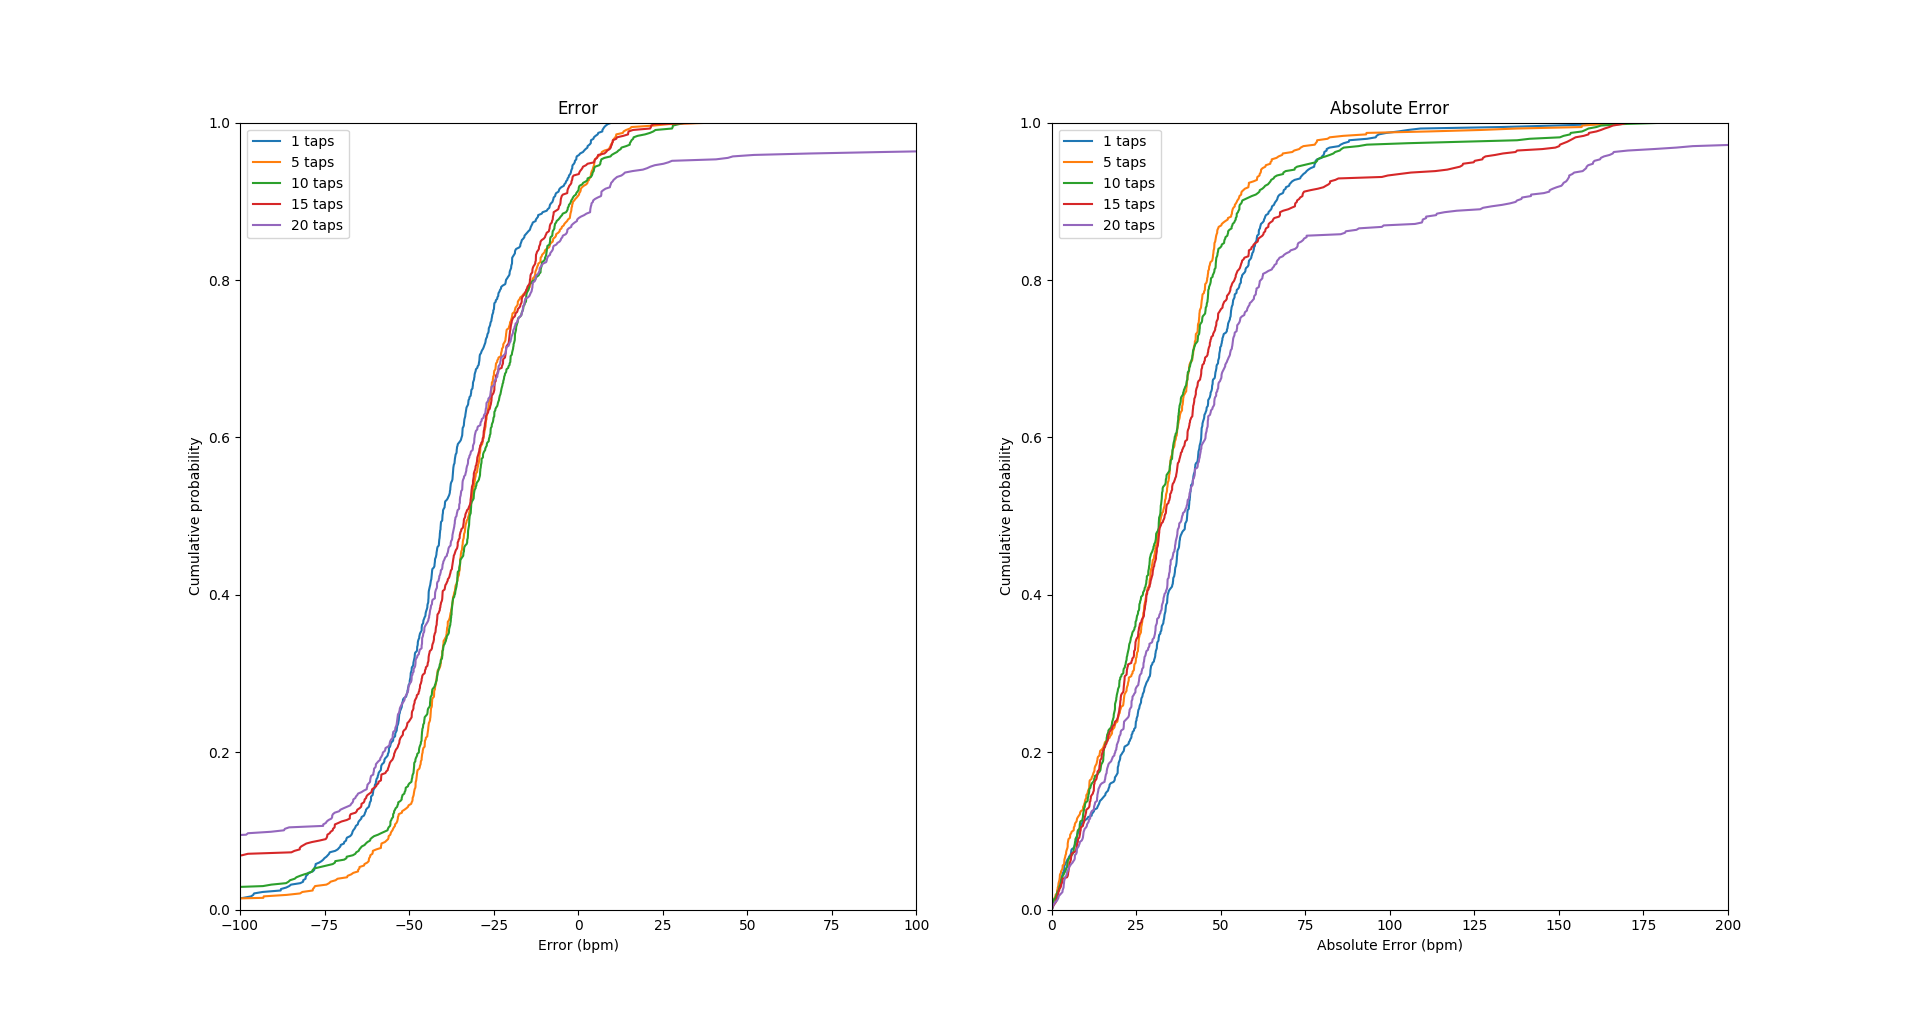
\includegraphics[width=0.9\textwidth]{figs/lms-taps-error-medium-noise.png}}
	\caption{Comparison of LMS Error at Different Tap Numbers.}
	\label{fig:lms-medium}
\end{figure}

The results show that all of the errors are skewed towards negative values,
regardless of number of taps, as all error plots are skewed to the left of the error=0
line. Looking at the absolute errors, we see that
using 15 taps produces the lowest median absolute error, as the curve remains
closest to error = 0. Having 1 tap produces a worse error, as we do not reduce
enough of the motion noise, whereas more taps removes too much data, resulting
in the error increasing.

Next, using 15 taps, I determine the best step value to use for LMS filtering.
I plot the cumulative graphs again, see figure \ref{fig:lms-medium-step}. The
results show all the step sizes under-approximate the heart-rate, however a
step size of $1$ provides the lowest absolute error, and hence should be used.
Lower step sizes likely take too long to converge, and don't reach the correct
solution, while larger step sizes likely miss the solution.

\begin{figure}[H]
	\centerline{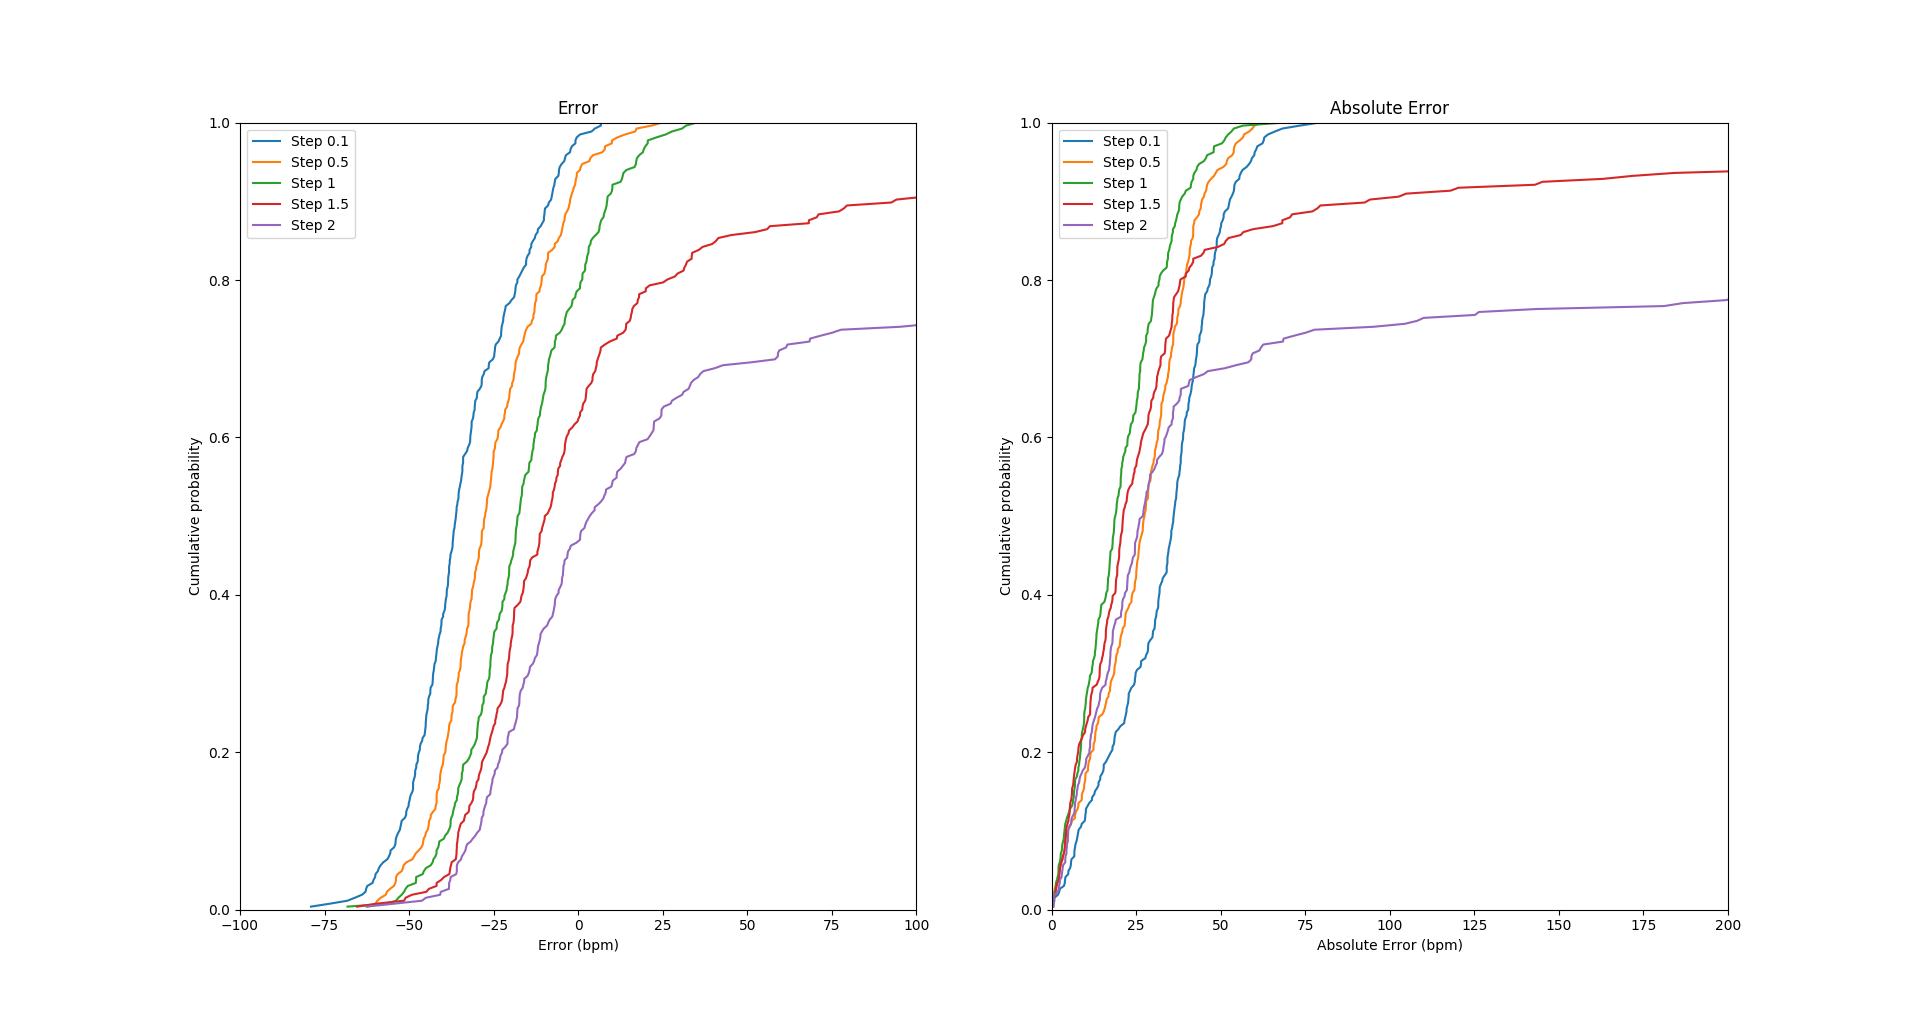
\includegraphics[width=0.9\textwidth]{figs/lms-steps-error-medium-noise.png}}
	\caption{Comparison of LMS Error at Different Step Sizes.}
	\label{fig:lms-medium-step}
\end{figure}


\subsection{NLMS}

To determine which axes to use, I run the same test as previously but using
NLMS instead. The results are in Table \ref{table:nlms-errors}. Again,
filtering using just the x-axis has a much lower average ordering than the
other techniques, so I will filter using just the x-axis from here on.

\begin{table}[]
\centering
\caption{Comparing NLMS Filtering with Different Axes.}
\label{table:nlms-errors}
\begin{tabular}{|l|l|l|l|}
\hline
X Filtering & Y Filtering & Z Filtering & Average Order \\ \hline
Y           & Y           & Y           & 4.68          \\
Y           & Y           & N           & 4.83          \\
Y           & N           & Y           & 2.95          \\
Y           & N           & N           & 1.83          \\
N           & Y           & Y           & 5.20          \\
N           & Y           & N           & 5.40          \\
N           & N           & Y           & 3.13          \\
\hline
\end{tabular}
\end{table}

Next I investigate the effect of the number of taps on NLMS. The results, in
figure \ref{fig:nlms-medium-taps}, are very similar to what we saw for LMS, and
again using 15 taps is optimal.
Now, I see how step size effects NLMS. The errors are plotted in
figure \ref{fig:nlms-medium-step}. We see that a step size of 1 is optimal,
any larger and very quickly the error increases as we don't converge on the
actual solution.

\begin{figure}[H]
	\centerline{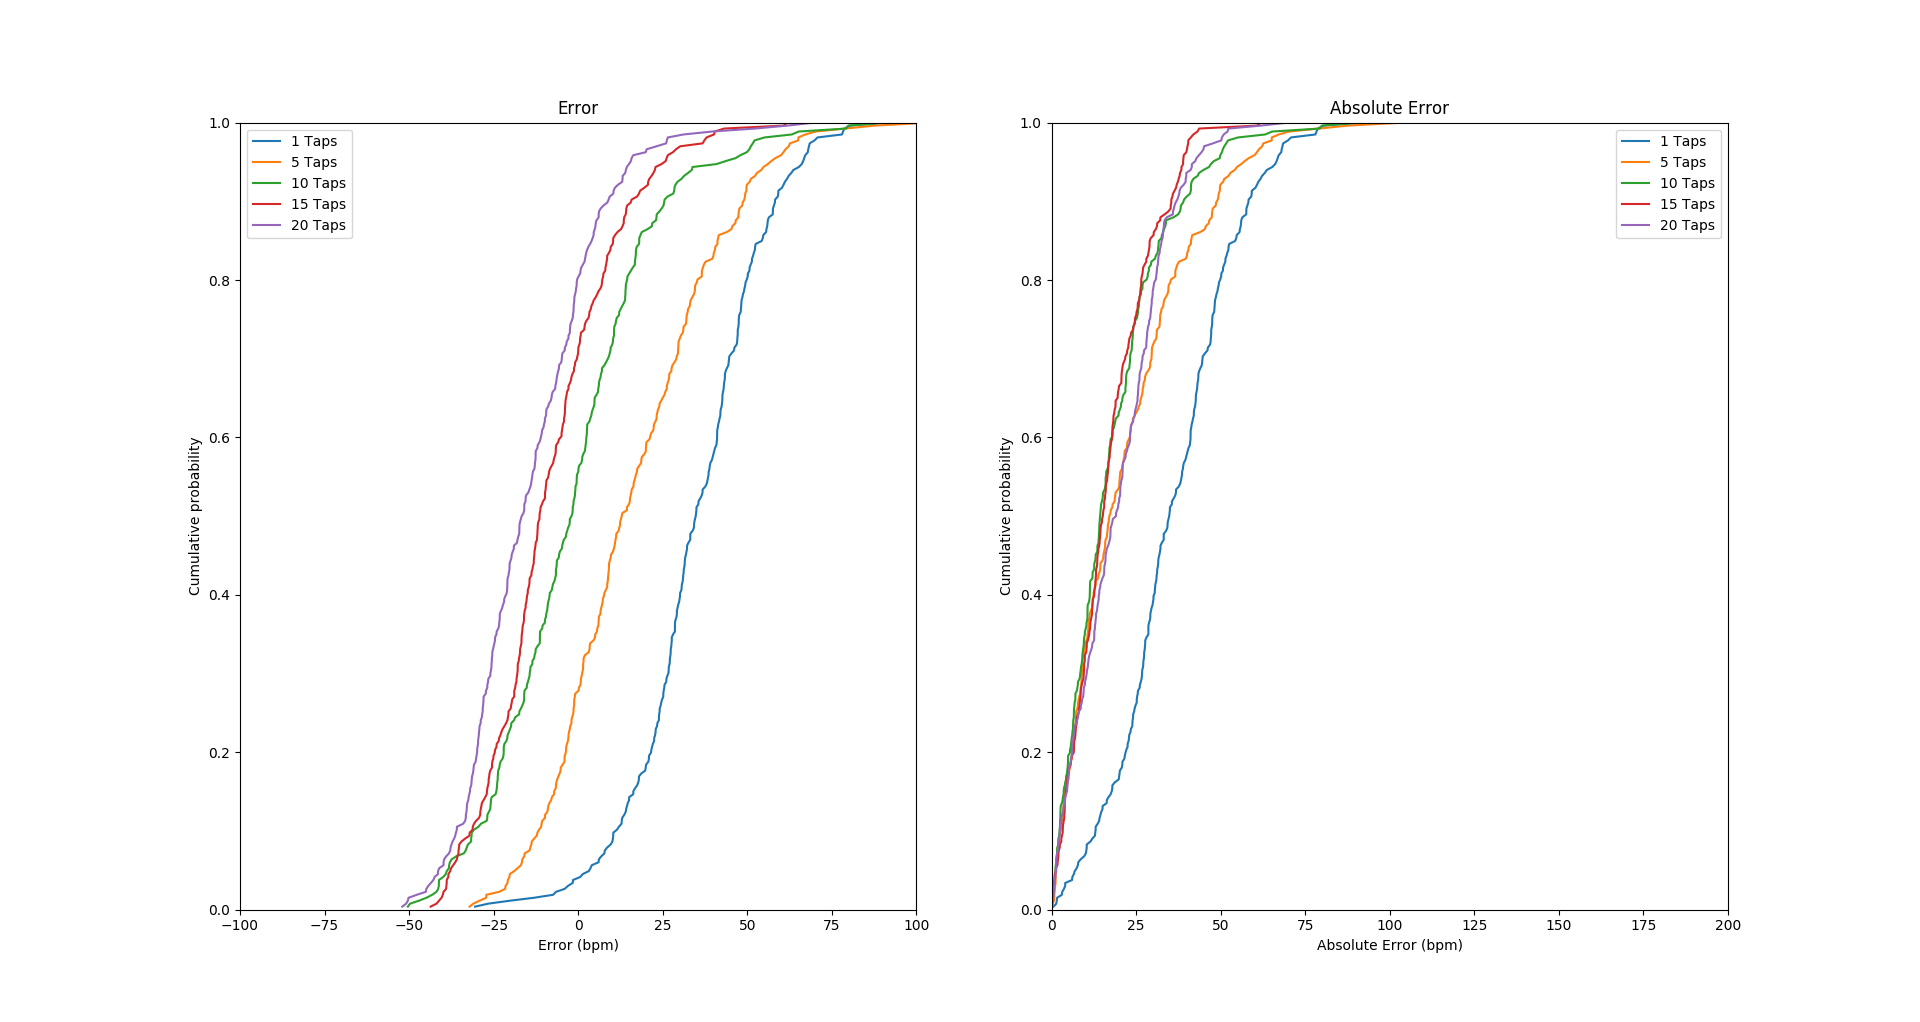
\includegraphics[width=0.9\textwidth]{figs/nlms-taps-error-medium-noise.png}}
	\caption{Comparing Numbers of Taps for NLMS.}
	\label{fig:nlms-medium-taps}
\end{figure}


\begin{figure}[H]
	\centerline{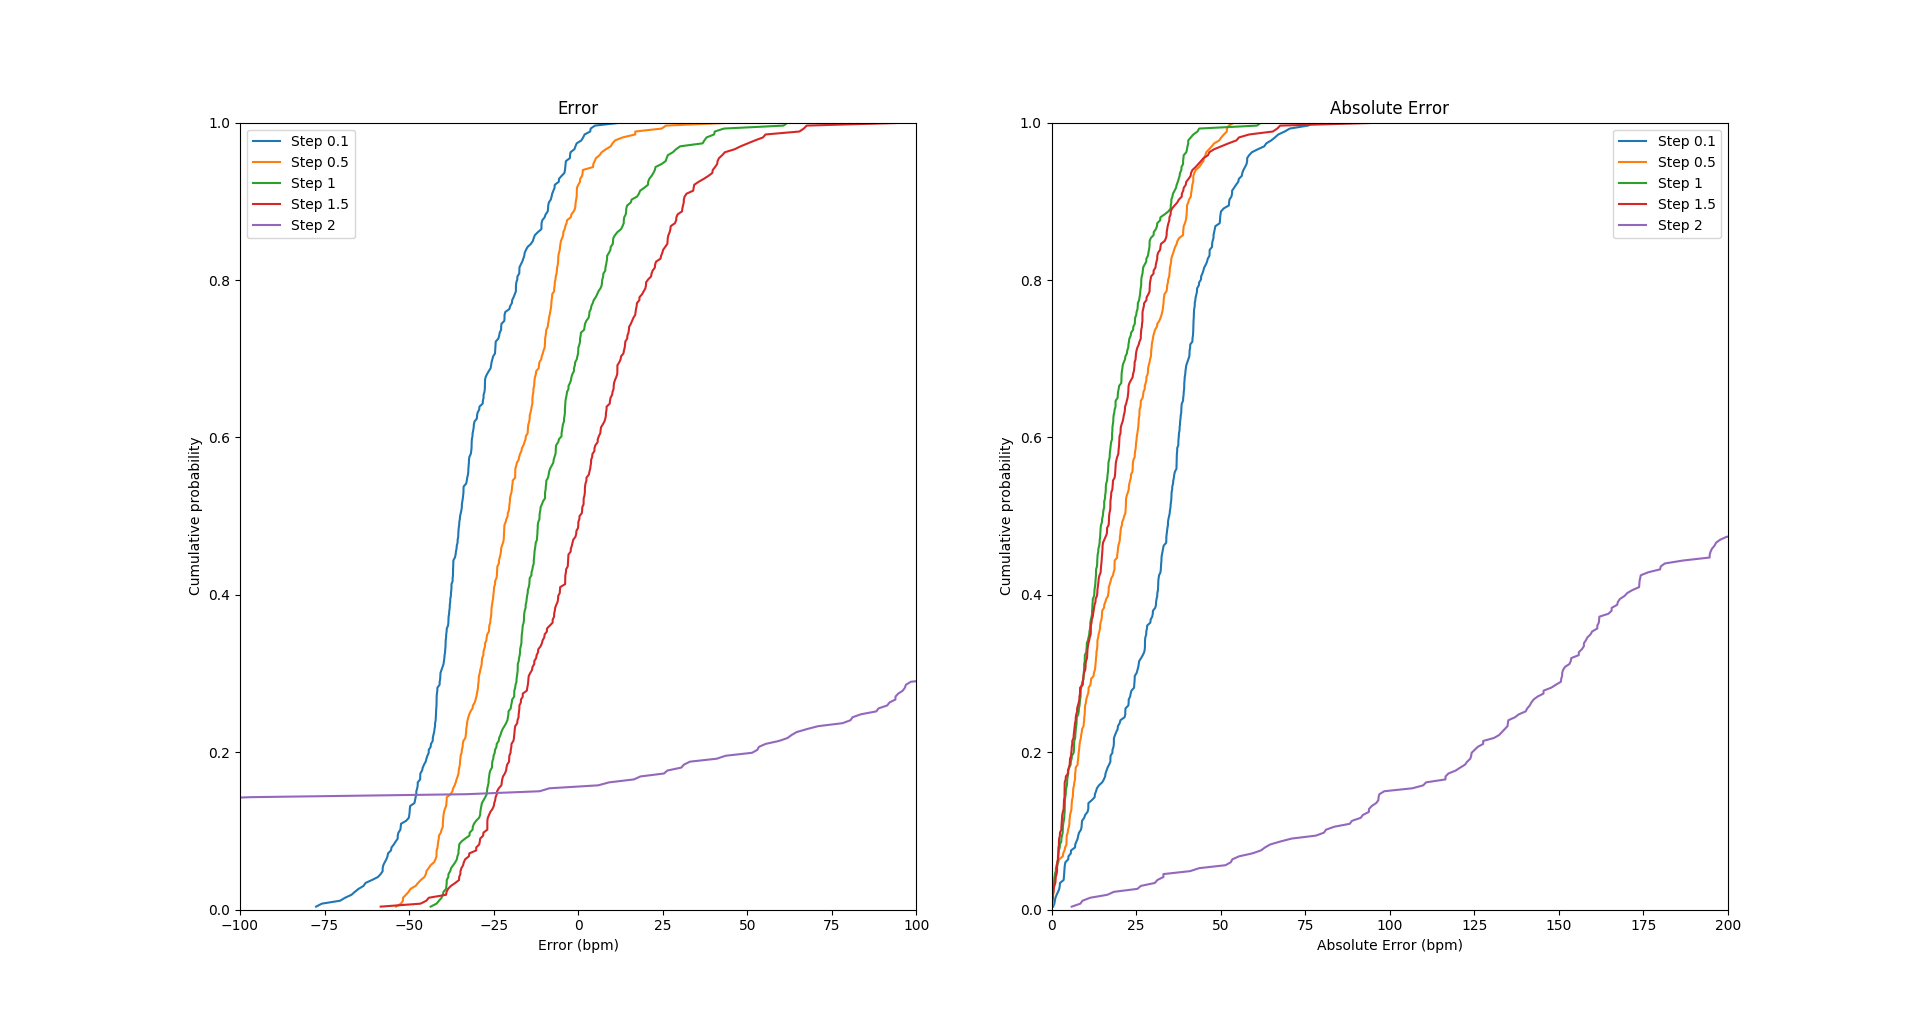
\includegraphics[width=0.9\textwidth]{figs/nlms-steps-error-medium-noise.png}}
	\caption{Comparing Step Size for NLMS.}
	\label{fig:nlms-medium-step}
\end{figure}

Now I have investigated LMS and NLMS, finding the optimal parameters. I
will next look at the differences between them given their optimal
parameters, both in terms of execution time and accuracy.

In figure \ref{fig:lms-nlms-validity} I plot the errors calculated by the
algorithms. The plot shows that they both tend to underestimate the
heart-rate. However, NLMS produces a slightly lower absolute error. 

\begin{figure}[H]
	\centerline{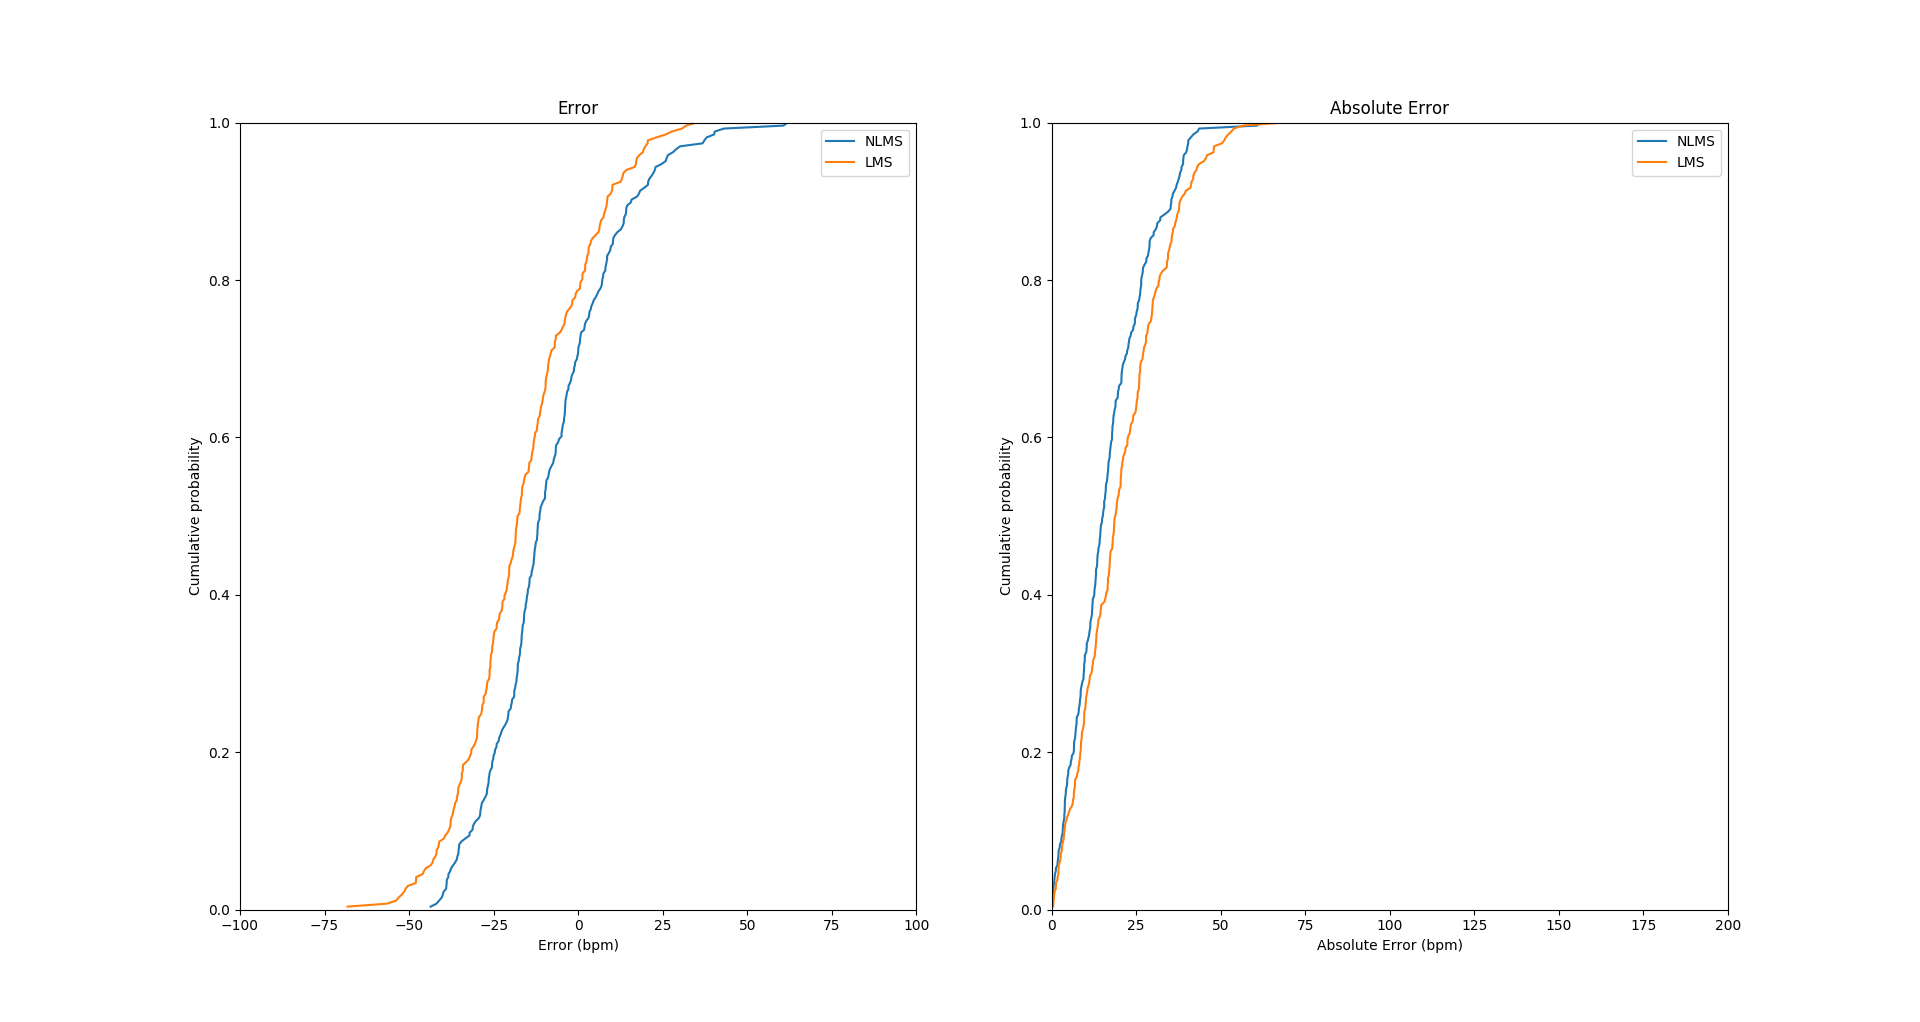
\includegraphics[width=0.9\textwidth]{figs/nlms-lms-validity.png}}
	\caption{Comparison of NLMS and LMS Accuracy.}
	\label{fig:lms-nlms-validity}
\end{figure}

To test time, I use the Python module \emph{timeit} to run the algorithms on
thirty seconds of data, and time how long they take to run 10000 times over.
The results are in table \ref{table:lms-nlms-time}, showing that lms runs in
less time than NLMS. Hence the choice between NLMS and LMS is a trade-off
between need for quick results and need for lower errors.

\begin{table}[H]
\centering
\caption{Comparing Adaptive Filtering Running Times.}
\label{table:lms-nlms-time}
\begin{tabular}{|l|l|}
\hline
Technique               & Time for 10000 iterations (s) \\ \hline
NLMS                    & 44.61                         \\
LMS                     & 34.49                         \\
\hline
\end{tabular}
\end{table}


\section{Heart Rate Calculation}

To evaluate my Heart-Rate calculation, I first calculate the running time of
both algorithms - local maxima, and peak-peak standard deviation minimization
. I also establish the effectiveness of the algorithms, when given a clean
PPG signal.

For the clean data, I have recorded an hour of data using the wristwatch and ECG
where I do not make large movements. I then pass it through a Butterworth filter to remove
noise out of the valid range. I don't do any adaptive filtering as
there should be minimal motion noise in this data.

First I evaluate the time taken, by running the algorithms on a section of
data which is 30 minutes long, and repeating 1000 times. I only run it on one
piece of data as the performance will be the same regardless of the data. 
As can be seen in Table \ref{table:hr-times},
the local maxima technique is much less expensive. This is as it only needs to
iterate through the signal once. Hence I should choose the local maxima
technique if it can perform as well as standard deviation minimization.

\begin{table}[]
\centering
\caption{Comparing Heart Rate Calculation Running Times.}
\label{table:hr-times}
\begin{tabular}{|l|l|}
\hline
Technique                       & Time for 1000 iterations (s) \\ \hline
Local Maxima                    & 0.36                         \\
Standard Deviation Minimisation & 76.54                        \\
\hline
\end{tabular}
\end{table}

Next I compare the result of the heart-rate calculation to the actual
heart-rate measure provided by the ECG.
In figure \ref{fig:hrc-error} I plot the error and absolute error of both
methods. The data clearly shows that standard deviation minimization is
superior, providing a much lower average absolute error. We see that 90\% of
the recorded errors are below 10bpm, whereas 90\% of local maxima calculated
heart-rates are below 35bpm. The error graph shows that the local maxima
technique nearly always over-approximates the heart-rate, whereas the standard
deviation technique tends to under-approximate.

\begin{figure}[H]
	\centerline{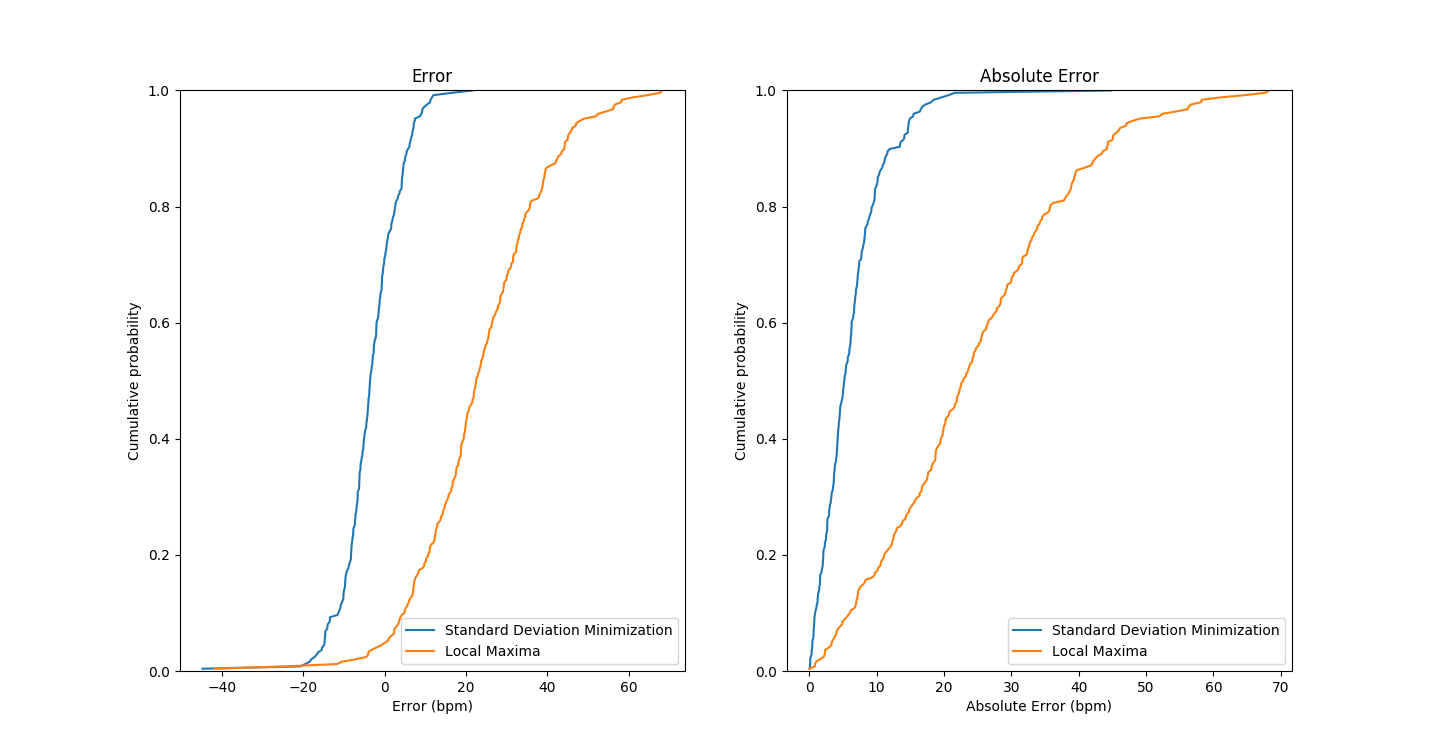
\includegraphics[width=1\textwidth]{figs/peakfind.png}}
	\caption{Comparison of Peak Finding Algorithms.}
	\label{fig:hrc-error}
\end{figure}

The reason the errors differ so much can be seen in figure
\ref{fig:hr-peak-comparison}. It is clear that the local maxima technique
over-approximates the number of peaks, as it often finds peaks which are
either noise or not caused by the heart-rate.

\begin{figure}[H]
	\centering
	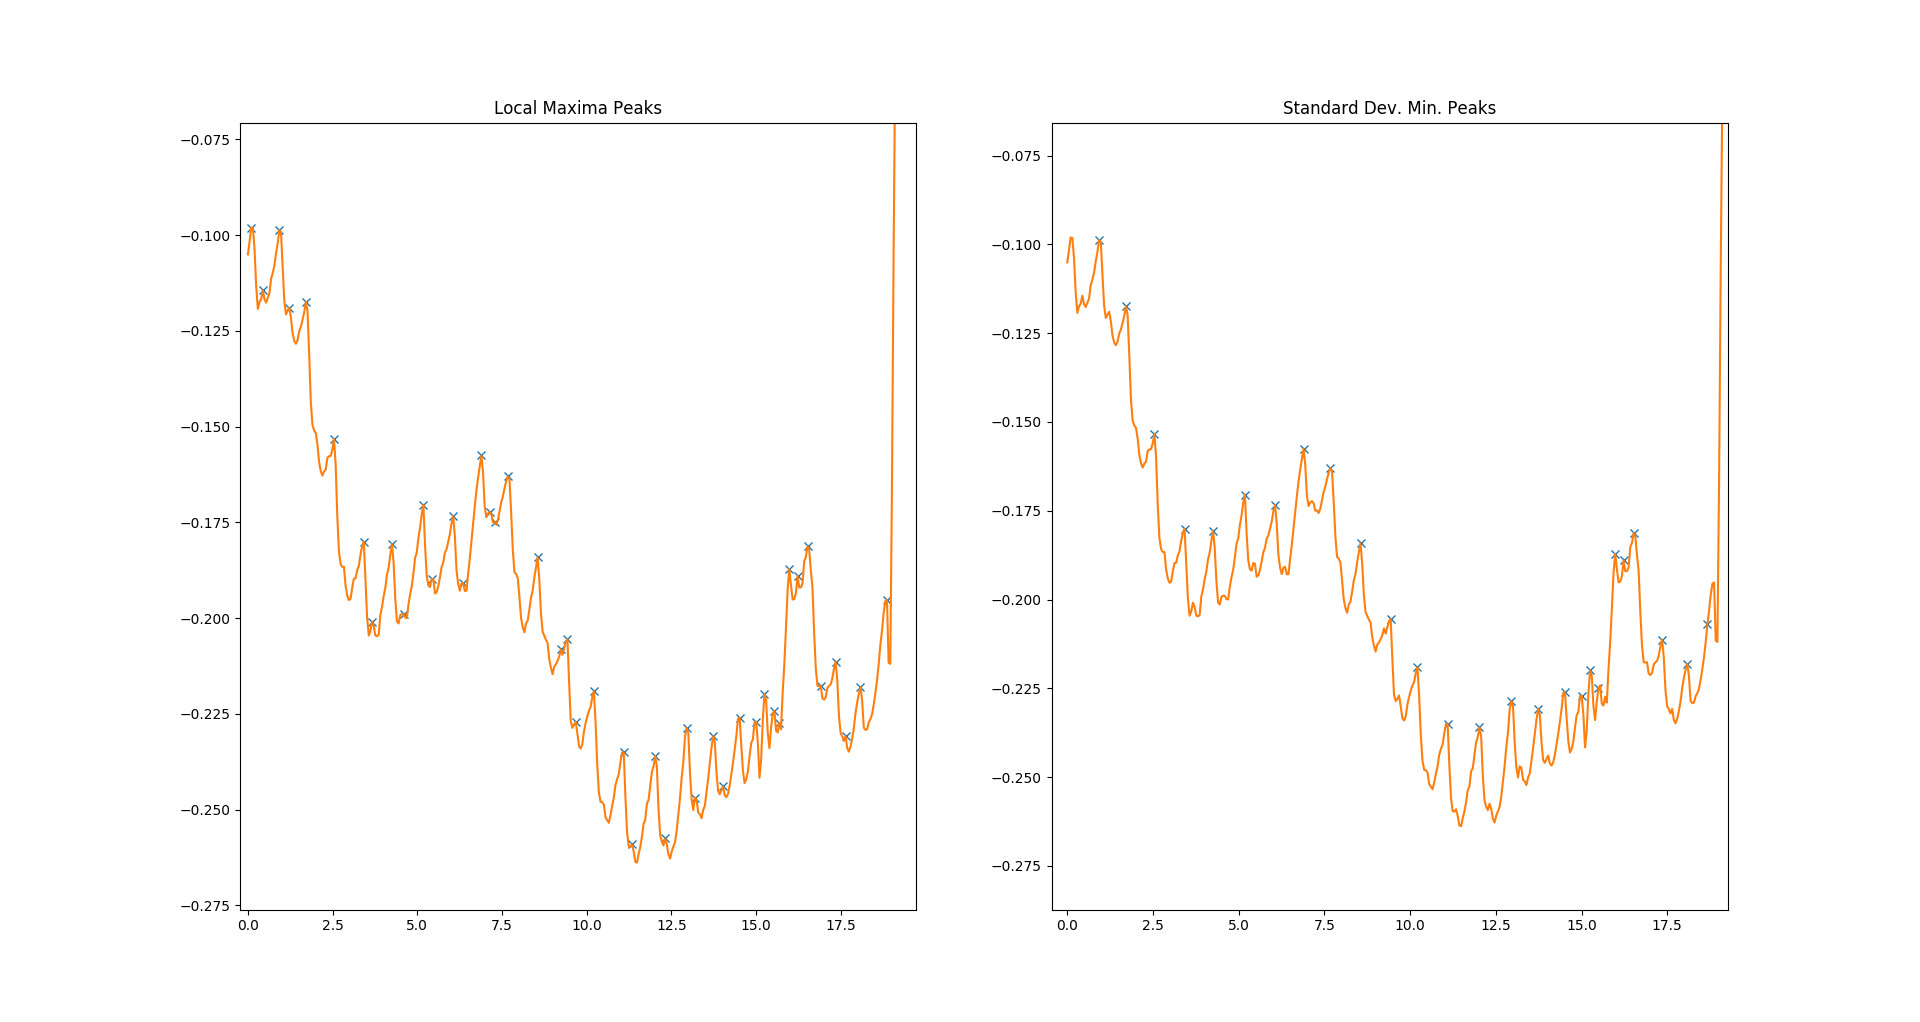
\includegraphics[width=1\textwidth]{figs/peak-comparison.png}
	\caption{Comparison of Heart Rate Peak Calculations.}
	\label{fig:hr-peak-comparison}
\end{figure}

I will use the standard deviation minimization technique in my work, as it
produces significantly lower errors. It does take longer, however it would
still produce results in real-time on a smart-watch.

\section{Joint Sparse Spectrum Reconstruction}

In this section I will evaluate my alternative algorithm developed in section
\ref{sec:joss}. I evaluate the spectral subtraction, then compare the
overall accuracy against NLMS.

To evaluate how effective spectral subtraction is for removing motion noise, I
run the algorithm on a run recorded at 9 kph, with and without subtraction.
The results are in figure \ref{fig:joss_eg} and show that without subtraction,
the algorithm locks into the wrong frequency, caused by a large motion
artefact. However, with spectral subtraction we find that the right bpm is
selected.

\begin{figure}[H]
\begin{subfigure}{.5\textwidth}
  \centering
  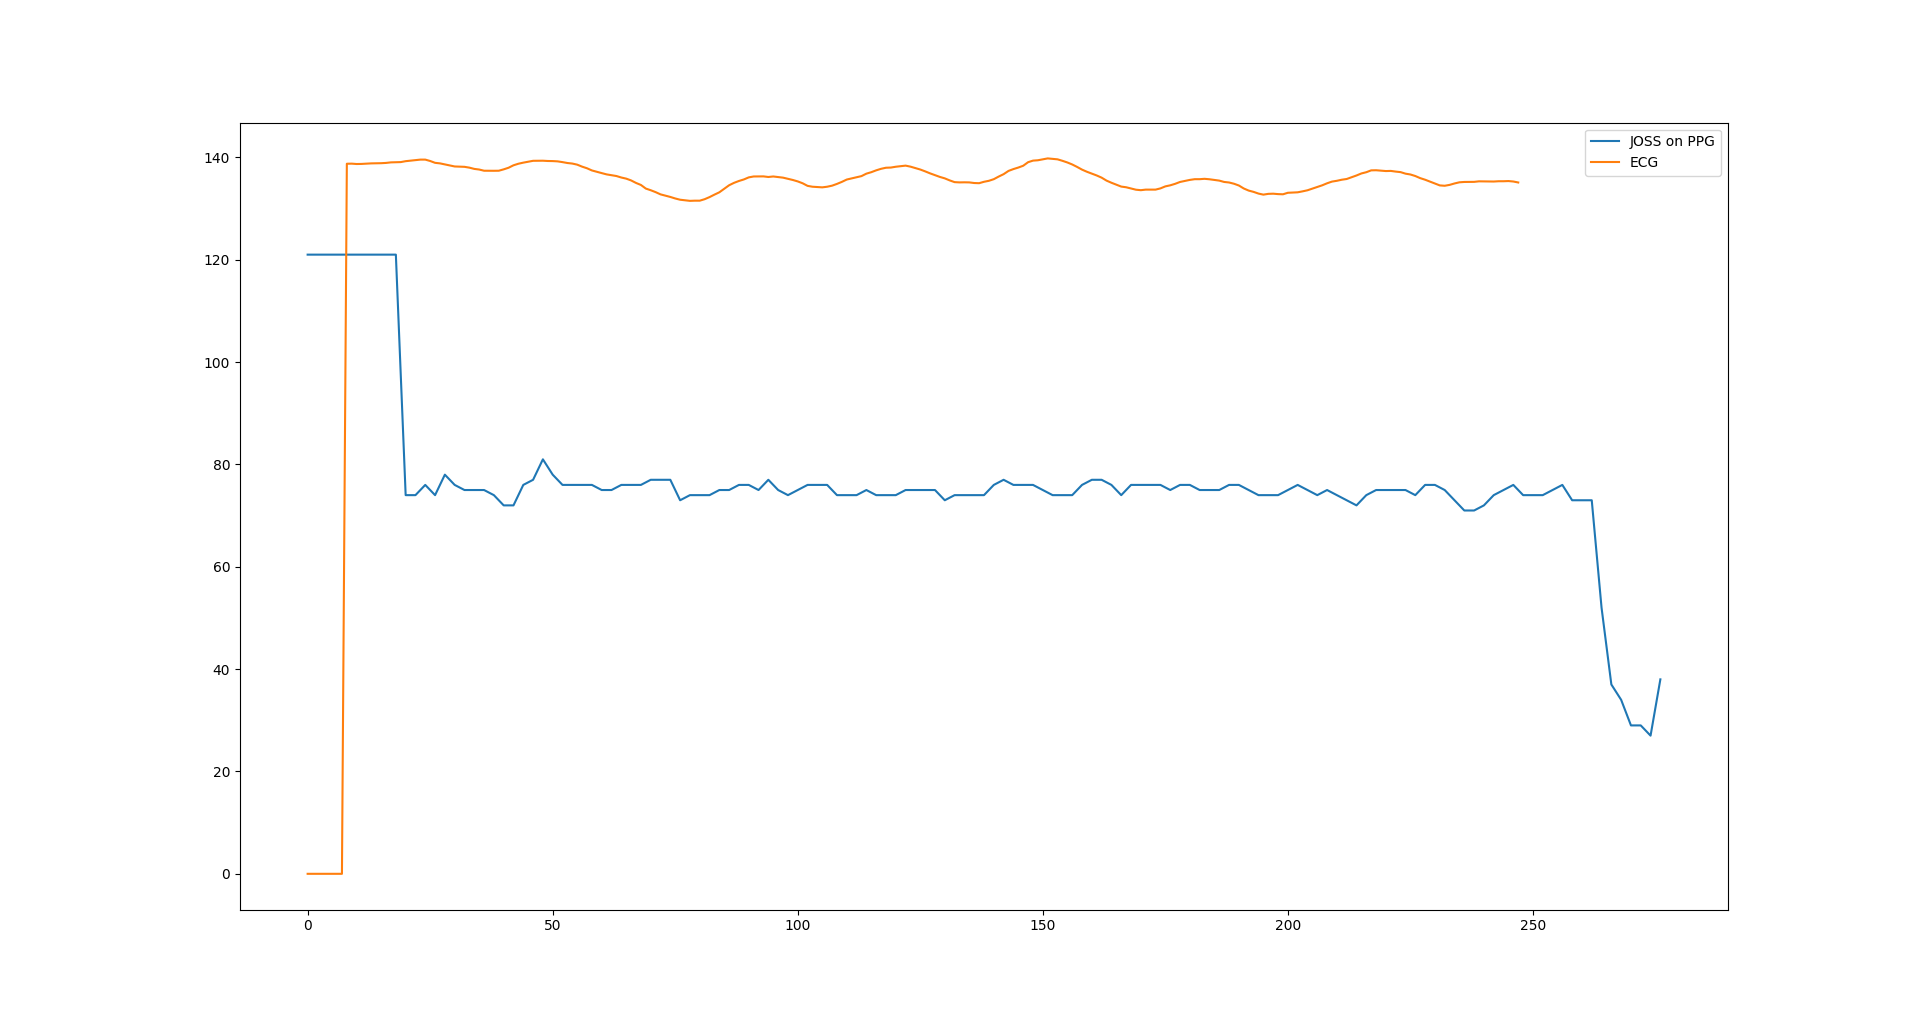
\includegraphics[width=\linewidth]{figs/joss_nosub.png}
  \caption{Without Subtraction.}
  \label{fig:joss_nosub}
\end{subfigure}%
\begin{subfigure}{.5\textwidth}
  \centering
  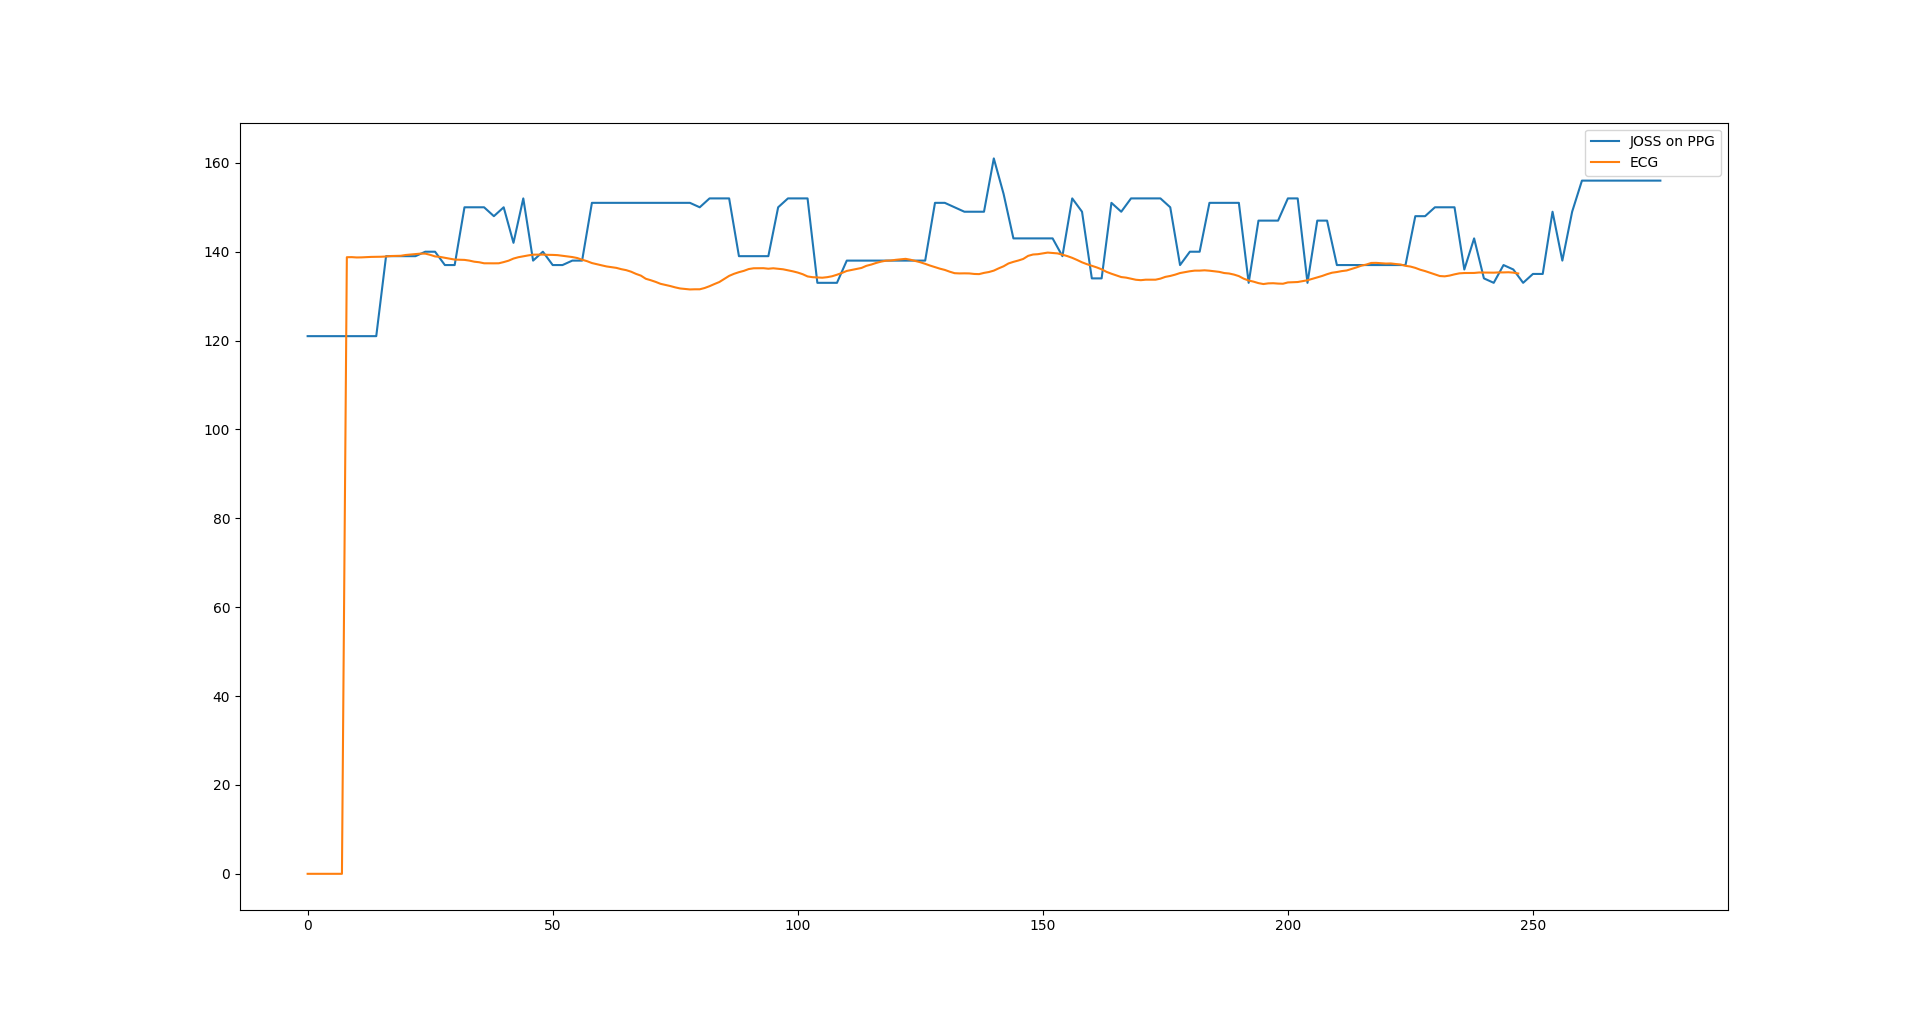
\includegraphics[width=\linewidth]{figs/joss_sub.png}
  \caption{With Subtraction.}
  \label{fig:joss_sub}
\end{subfigure}
\caption{Spectrum Reconstruction.}
\label{fig:joss_eg}
\end{figure}

I next plot the errors, see figure \ref{fig:joss_nlms}, comparing the spectrum
reconstruction to NLMS, for samples taken with both high and low motion noise. 

With low motion noise, NLMS is significantly better than spectrum
reconstruction. I estimate this is due to the spectrum subtraction - small
movements result in large and random fluctuations in the accelerometer's
spectrum - which may then be subtracted from the PPG, removing the useful
signal. 

With approximately 30\% of the high motion noise, spectrum reconstruction
performs better than NLMS, these are the cases where the correct frequency is
tracked. However, for the remaining data, NLMS is far better. The error plot
shows that for about 50\% of the data, spectrum methods produce a heart-rate between
125 and 150 bpm lower than the ECG. This is likely caused by the algorithm
locking on to a lower frequency, such as motion noise - evidence that the
spectrum subtraction is not completely effective.

\begin{figure}[H]
\centering
\begin{subfigure}{.85\textwidth}
  \centering
  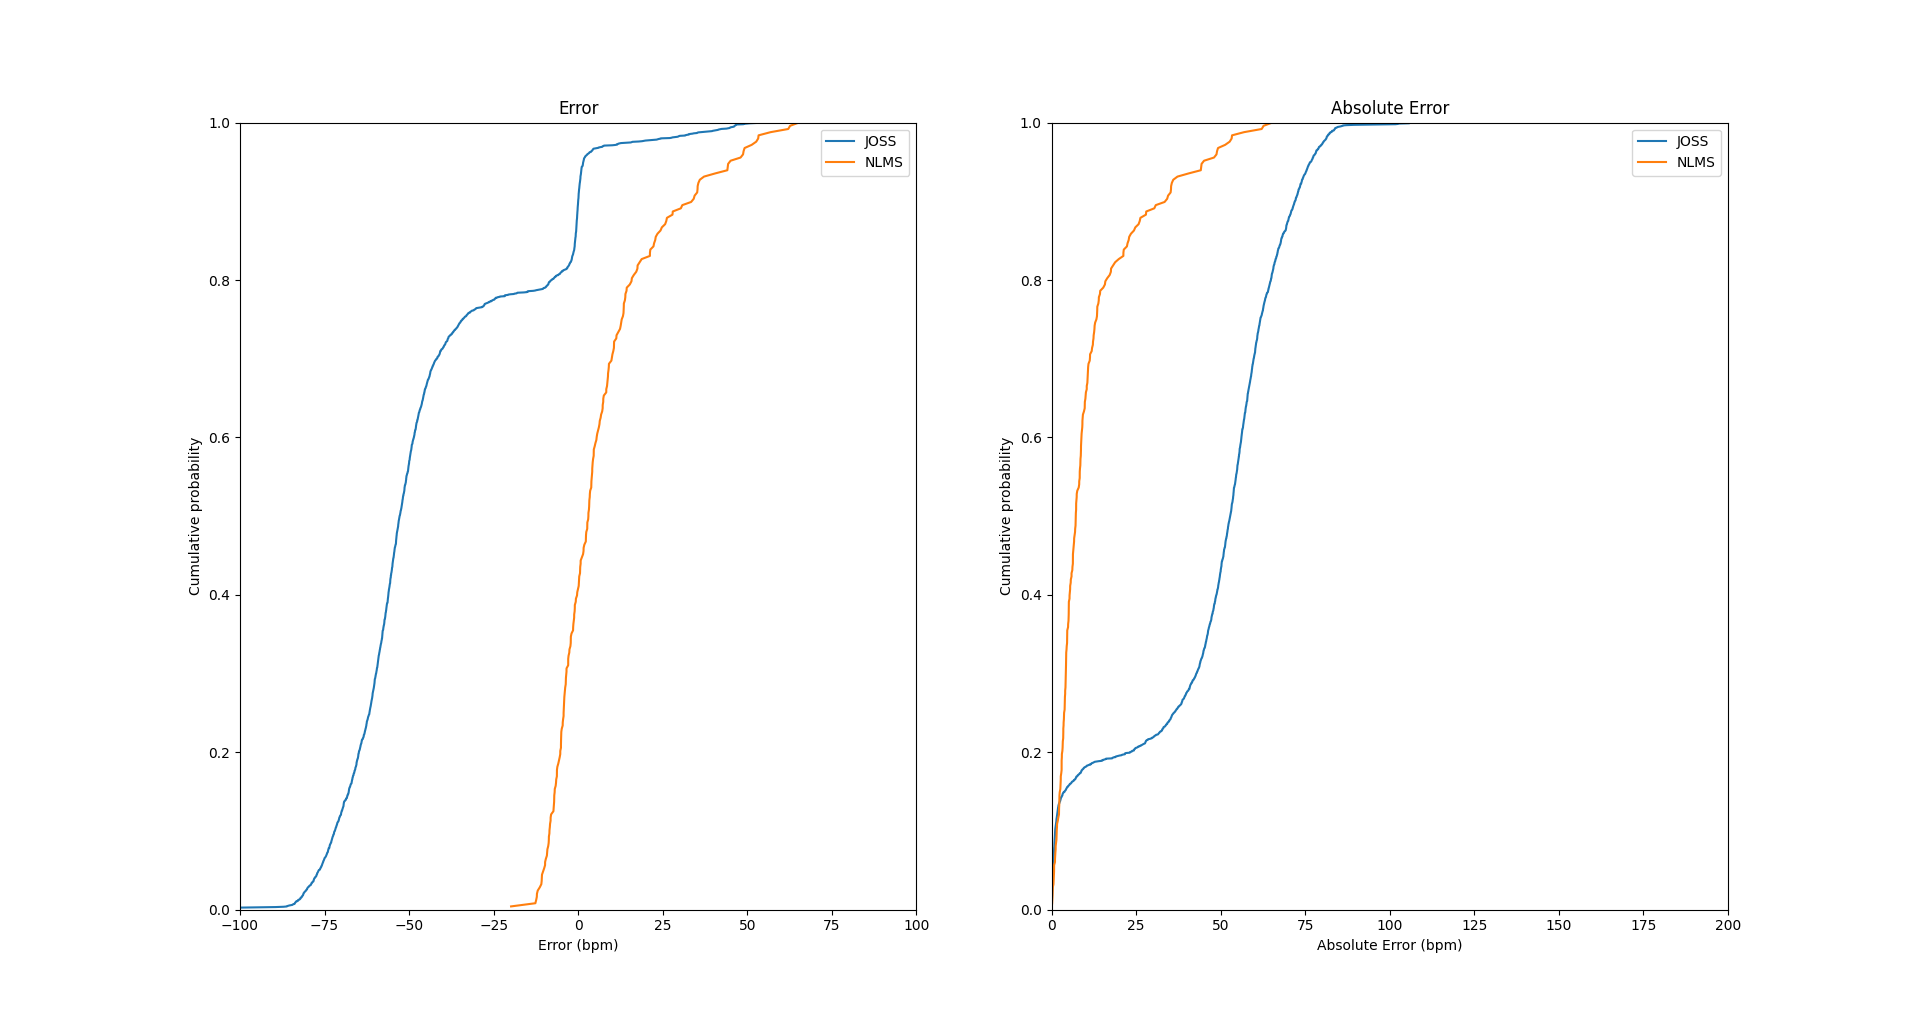
\includegraphics[width=\linewidth]{figs/joss_nlms_low.png}
  \caption{Low Motion Noise.}
  \label{fig:joss_nlms_low}
\end{subfigure}
\\
\begin{subfigure}{.85\textwidth}
  \centering
  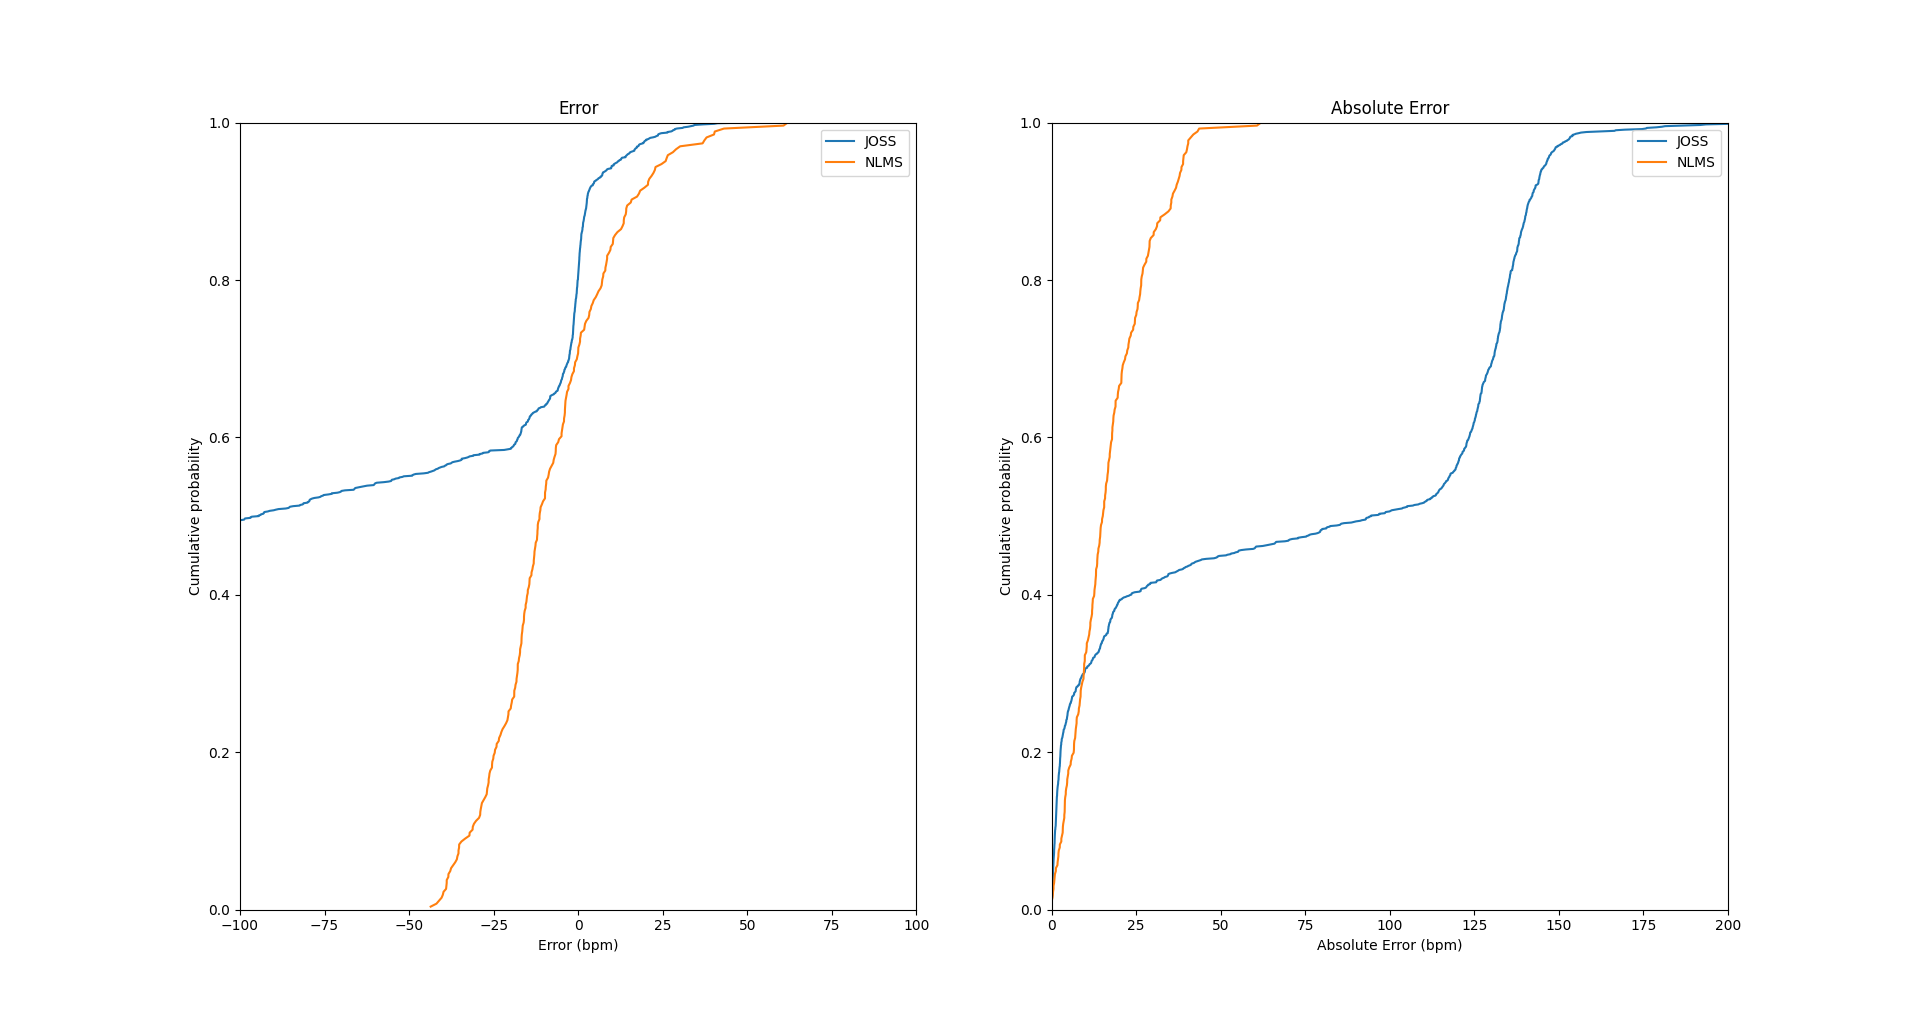
\includegraphics[width=\linewidth]{figs/joss_nlms_medium.png}
  \caption{High Motion Noise.}
  \label{fig:joss_nlms_medium}
\end{subfigure}
\caption{Comparing Spectrum Reconstruction to NLMS.}
\label{fig:joss_nlms}
\end{figure}

In conclusion, my NLMS method is preferable to the spectrum method, as it
produces far better results. The spectrum method requires more optimisation to
ensure that we never lock on to frequencies coming from noise.

\section{Earbuds}

In this section, I evaluate the performance of the earbuds alone, and then
evaluate some of the fixes I propose to issues identified in the evaluation.

The first step I took when evaluating the earbuds was to go on a fast run,
which would introduce much motion noise on the watch. You can see the
heart-rate from the earbuds plotted against the heart-rate I received from the
ECG in figure \ref{fig:earbud-fast}. The results are promising, with
heart-rate accurately tracked however there is an issue.

\begin{figure}[H]
	\centerline{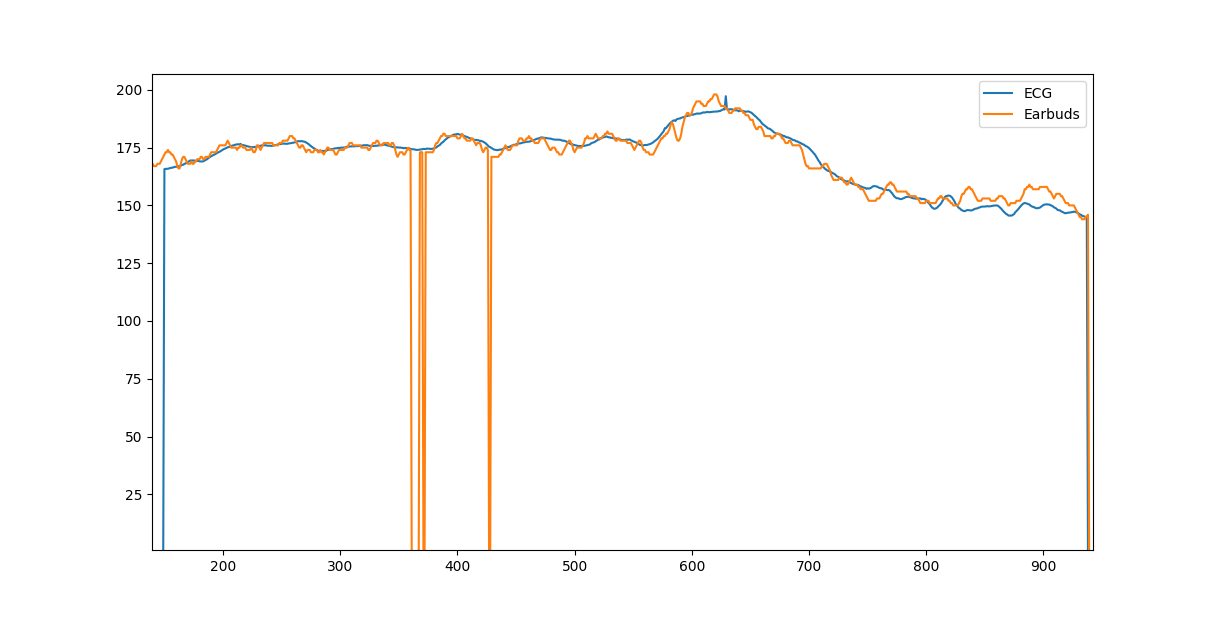
\includegraphics[width=0.9\textwidth]{figs/earbud-fast-graph.png}}
	\caption{Plot of Earbud Heart-rate against ECG.}
	\label{fig:earbud-fast}
\end{figure}

\subsection{Problem} \label{sec:earbud-problem}

The problem with the earbuds is that they occasionally lose contact with the
ear. This can happen as a combination of sweating and motion dislodges the
earbud. In addition, I found when running I would often have to stop and
adjust the earbud as I suspected it was going to fall out. 

The earbuds are quite sensitive to location, so if they become dislodged or
are rotated, the reported heart-rate drops to zero, as seen in figure
\ref{fig:earbud-fast} at $t=360, 375, 420$.

\subsection{Sensor Fusion}

Figure \ref{fig:kalman-working} shows the effectiveness of the Kalman filter -
when the earbud's signal drops out it follows the curve picked up by the
watch sensor.

\begin{figure}[H]
	\centerline{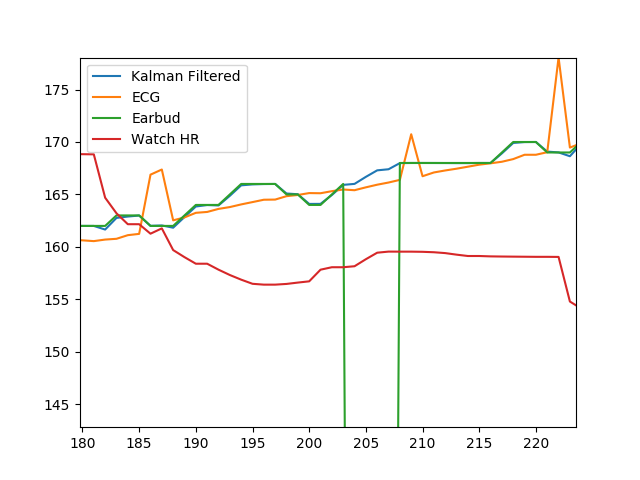
\includegraphics[width=0.7\textwidth]{figs/kalman-working.png}}
	\caption{Kalman Filter Demonstration.}
	\label{fig:kalman-working}
\end{figure}

In figure \ref{fig:kalman_error} we plot the errors for the watch sensor, the
earbud sensor and the sensor fusion technique. The graph shows that the
earbuds and hence the fusion technique produce a significantly lower error than the watch for 90\% of the
samples, as expected. And, for the 10\% the watch is better - as the earbuds
report 0 bpm. The sensor fusion technique is clearly better than the earbuds
for these samples as well, using the watch to guide the output. Hence, the
sensor fusion technique gets the best of both worlds.

\begin{figure}[H]
	\centerline{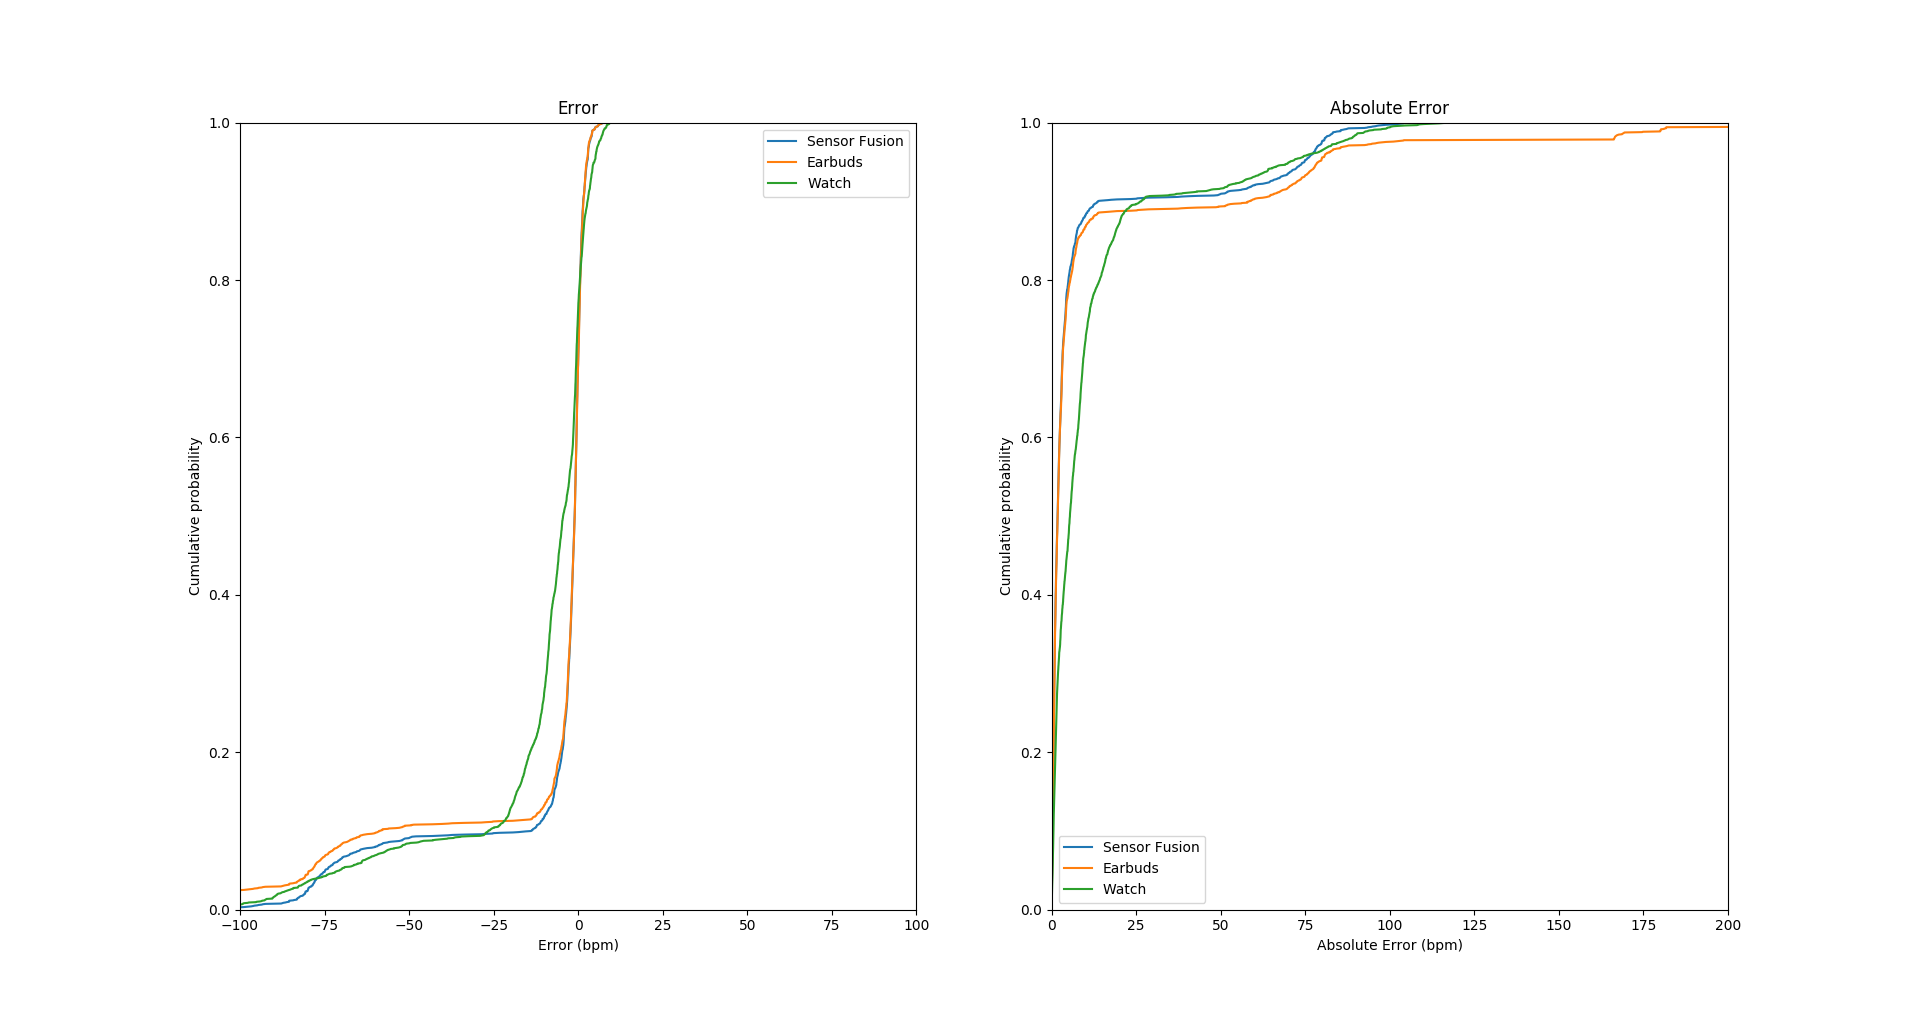
\includegraphics[width=0.9\textwidth]{figs/kalman_validity.png}}
	\caption{Sensor Fusion Error.}
	\label{fig:kalman_error}
\end{figure}

In this section I have shown that earbuds produce a very accurate signal, but
require the sensor fusion method I developed in order to avoid issues where
the rate drops to zero due to lack of contact.

\chapter{Conclusion}

I have met all the success criteria set out in my project proposal.
Additionally I have completed two extensions.

\paragraph{Summary}

In this project I explored a few techniques which calculate heart-rate from
the noisy signals coming from a smart-watch worn while running. To remove
random noise not caused by motion, I experimented with band-pass filters,
finding the optimal parameters for my usage. To remove motion noise, I
investigated and implemented two adaptive noise cancellation techniques. Then
to calculate the heart-rate I looked into two different methods. I also
looked at using joint spectrum calculations to estimate heart-rate and remove
motion noise, as an extension.

Finally, as an extension I showed that putting heart-rate sensors into earbuds is a promising
technique, although the signal can cut out. Hence, my developed sensor fusion
technique which combines heart-rate from the earbuds and from a wrist-watch
provides a better signal than either alone.

\paragraph{Issues}

I found that using the wrist watch sensors alone, I could not get a 
good estimate of heart-rate. This is in line with other algorithms suggested
in papers.

Using spectrum reconstruction appears to be effective in some cases but can
latch on to the wrong frequency and never recover the correct signal. In
future work, some more research might be done into determining whether the
frequency we're currently tracking is reasonable.

Using two sensors, I found I could estimate heart-rate with much more
confidence. Currently the sensor-fusion algorithm is not very accessible to
users, as the interface is very minimal, so if I had more time I would have
developed an interface which allowed users to better track their workouts.




%%%%%%%%%%%%%%%%%%%%%%%%%%%%%%%%%%%%%%%%%%%%%%%%%%%%%%%%%%%%%%%%%%%%%
% the bibliography
\addcontentsline{toc}{chapter}{Bibliography}
\bibliography{refs}

%%%%%%%%%%%%%%%%%%%%%%%%%%%%%%%%%%%%%%%%%%%%%%%%%%%%%%%%%%%%%%%%%%%%%
% the appendices
\appendix
\chapter{}
\section{Repository Overview}\label{app:repo_overview}
\tiny
\begin{forest}
  for tree={
    font=\ttfamily,
    text width=\textwidth,
    grow'=0,
    child anchor=west,
    parent anchor=south,
    anchor=west,
    calign=first,
    edge path={
      \noexpand\path [draw, \forestoption{edge}]
      (!u.south west) +(7.5pt,0) |- node[fill,inner sep=1.25pt] {} (.child anchor)\forestoption{edge label};
    },
    before typesetting nodes={
      if n=1
        {insert before={[,phantom]}}
        {}
    },
    fit=band,
    before computing xy={l=15pt},
  }
[
  [{\bf ppg-recorder/app/src} - Contains Android project designed for the
	  watch
	  [\emph{EarHRRecorder.kt} - Controls recording HR from bluetooth
	  earbuds]
	  [\emph{GattAttributes.kt} - Defines constants used in
	  Bluetooth-LE]
	  [\emph{HeartDeviceScanListener.kt} - Used to search for Bluetooth
	  devices]
	  [\emph{HeartDeviceService.kt} - The service which listens for
	  updates from Bluetooth updates in the background]
	  [\emph{MainActivity.kt} - Runs the main thread of the program]
	  [\emph{PpgRecorder.kt} - Records data from the watch's PPG sensor]
	  [\emph{SaveListener.kt} - Provides feedback once data is saved to
	  filesystem]
	  [\emph{SensorRecorder.kt} - Parent class for all sensor recorders]
	  [\emph{Sync.kt} - Uploads recorded data to a server]
  ]
  [{\bf server} - A server to run on a raspberry pi and receive data
	  [\emph{gdrive.py} - Uploads files to Google Drive]
	  [\emph{server.py} - Server code built with Flask]
  ]
  [{\bf data} - Contains files to process the recordings in addition to the recorded data
    [\emph{data.py} - Code used to represent signals] 
    [\emph{earbuds.py} - Used to represent signals from the earbuds]
    [\emph{ecgdata.py} - Used to represent signals from the ECG]
    [{\bf evaluation} - Programs used to evaluate the project
      [\emph{correlationtest.py} - Used to verify informed correlation results]
      [\emph{earbud\_test.py} - Used to test sensor fusion techniques]
      [\emph{filtertest.py} - Used to test filtering algorithms]
      [\emph{josstest.py} - Used to test the JOSS-based algorithm]
      [\emph{motionfiltertest.py} - Used to test LMS and NLMS]
      [\emph{peakfindtest.py} - Used to test peakfinding code]
      [\emph{syncstest.py} - Used to split data into segments based on speed]
    ]
    [\emph{filtering.py} - Runs a butterworth and chebyshev filter]
    [\emph{heartrate.py} - Calculates heartrate when given the watch and ECG
    data]
    [\emph{joss.py} - Runs spectrum reconstruction on watch data]
    [\emph{kalmanfilter.py} - Implementation of Kalman filter]
    [\emph{MFOCUSS.m} - Implementation of MFOCUSS from \cite{ZhangCodes}]
    [\emph{motionfilter.py} - Implementation of LMS and NLMS]
    [\emph{peakfind.py} - Naive and sd-minimisation peakfinding functions]
    [\emph{sync.py} - Code which combines watch and ECG data ensuring they start at
    the same time]
    [\emph{watchdata.py} - Code to extract watch data]
  ]
]
\end{forest}
%\chapter{Data tables}
%\section{NLMS Absolute Errors} \label{section:nlms-errors}
%
%\csvautolongtable{figs/nlms_validity.csv}
%
%\section{LMS Absolute Errors} \label{section:lms-errors}
%
%\csvautolongtable{figs/lms_validity.csv}

\section{Project Proposal}

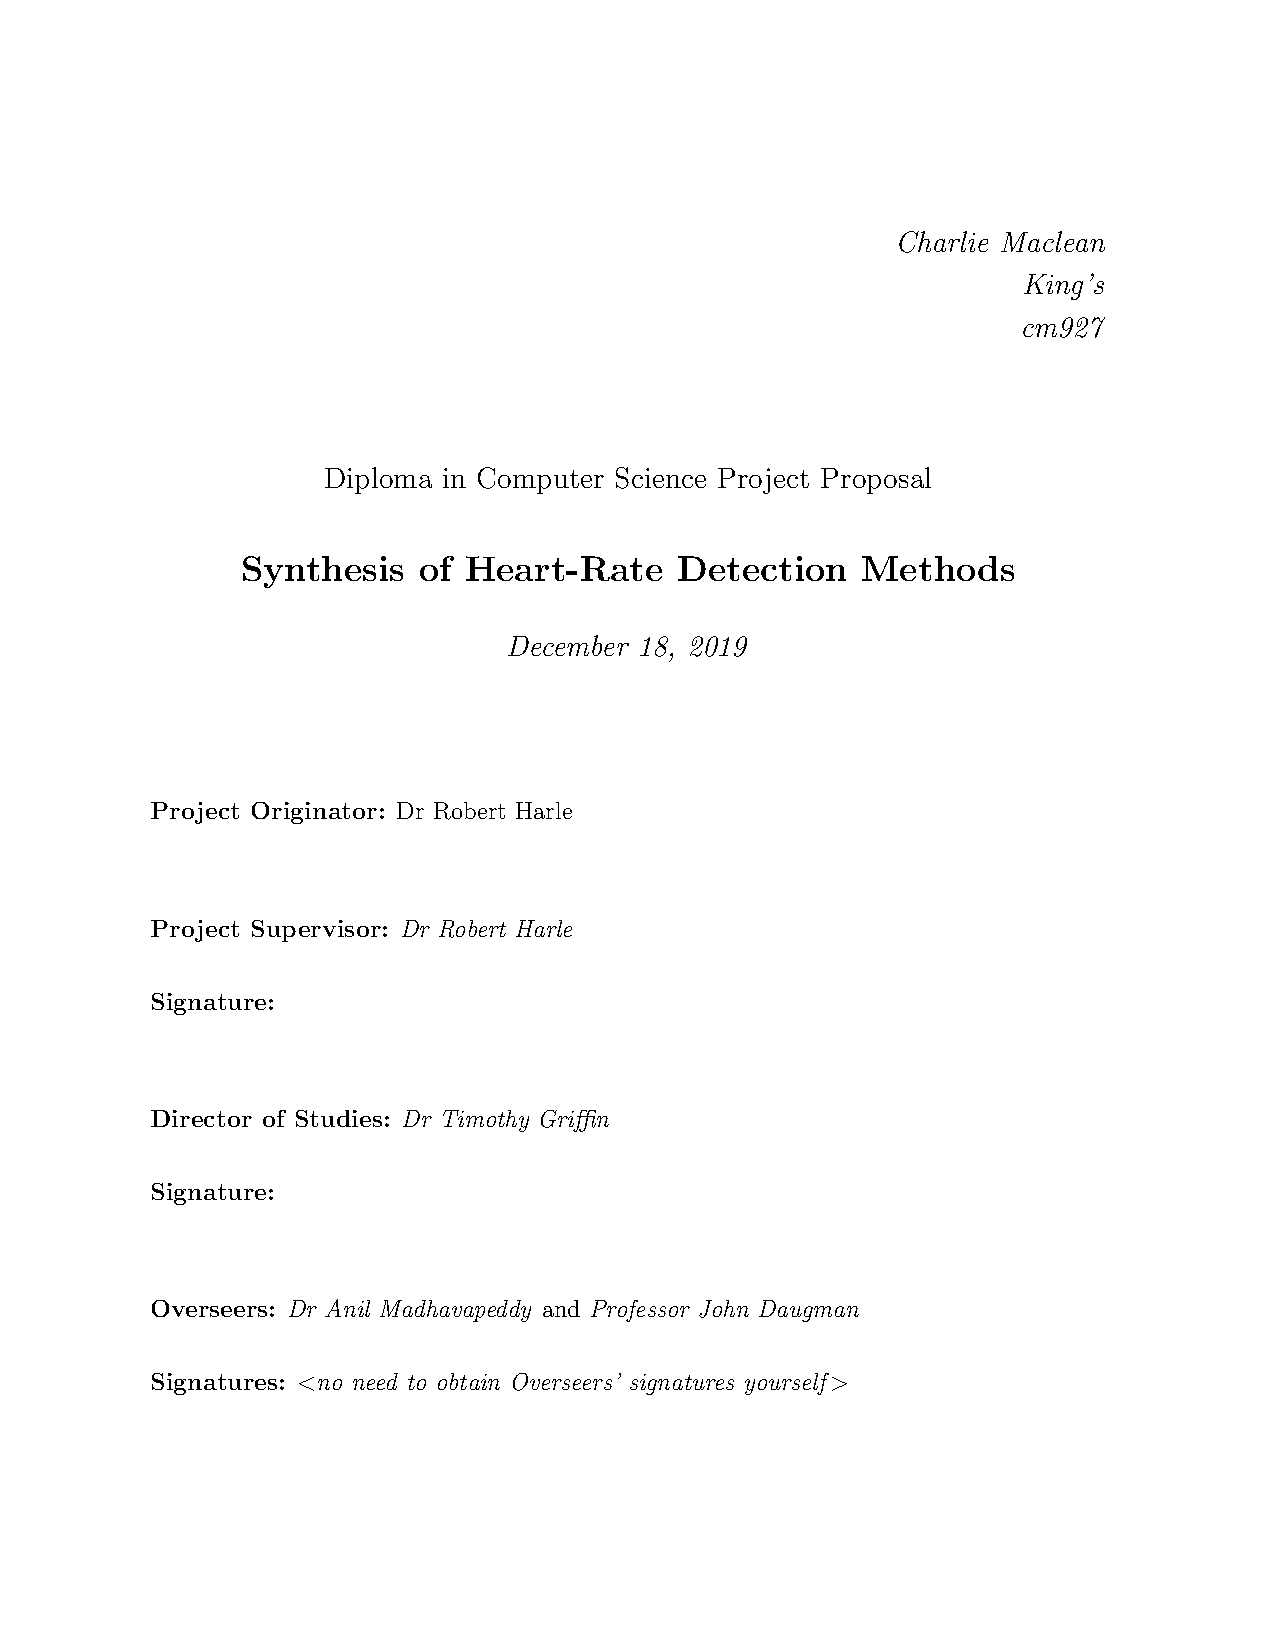
\includepdf[pages=-,pagecommand={},width=\textwidth]{proposal.pdf}

\end{document}
